\documentclass[times,english,12pt,oneside]{article}
% The preceding line is only needed to identify funding in the first footnote. If that is unneeded, please comment it out.

\usepackage{cite}
\usepackage{amsmath,amssymb,amsfonts}
\usepackage{algorithm}
\usepackage[noend]{algpseudocode}
\usepackage{graphicx}
\usepackage{textcomp}
\usepackage{xcolor}
\usepackage[nolist,nohyperlinks]{acronym}
\usepackage{lipsum}  
\usepackage{float}
\usepackage{bm}
\usepackage{subfigure} 
\usepackage{flushend}
\usepackage{cuted}
\usepackage{wrapfig}
\usepackage{rotating}
\usepackage{bbm}
\usepackage{breqn}
%\usepackage{algorithm}
\usepackage[utf8x]{inputenc}
\usepackage{tikz}
\usepackage{enumerate}
\usepackage{multirow}
\usepackage{array}
\usepackage{colortbl}
\usepackage{algorithm}
\usepackage{verbatim}
\usepackage{url}
\usepackage{setspace}
\usepackage{geometry}
\usepackage[shortlabels]{enumitem}
\geometry{verbose,a4paper,tmargin=2.54cm,bmargin=2.54cm,lmargin=3.00cm,rmargin=2.04cm}
%\usepackage{hyperref}
% \usepackage{unicode-math}
% \setmainfont{Latin Modern Roman}
% \setmathfont{Latin Modern Math}

% \Umathchardef\xnot="3 \symoperators "0338
% \AtBeginDocument{\renewcommand\not[1]{#1\xnot}
% \renewcommand{\notin}{\in\xnot}}
%\usepackage{epstopdf}
\definecolor{LightBlue}{rgb}{0.67,0.847,0.9}
\definecolor{LightOrange}{rgb}{1,0.84,0.60}
\definecolor{LightGrey}{rgb}{0.9,0.9,0.9}

\newcommand{\secBest}[1]{\cellcolor{LightBlue}{#1}}
\newcommand{\best}[1]{\cellcolor{LightOrange}{#1}}
\newcommand{\todo}[1]{\textcolor{red}{TODO: #1}}
\newcommand{\niloy}[1]{\textcolor{red}{NG: #1}}
\newcommand{\basabdatta}[1]{\textcolor{blue}{BP: #1}}
\newcommand{\jay}[1]{\textcolor{green}{Jay: #1}}
\newcommand{\bs}[1]{\textcolor{purple}{#1}}
\newcommand{\new}[1]{\textcolor{blue}{#1}}
\newcommand{\ti}[1]{\textit{#1}}
\newcommand{\mq}[1]{$`{#1}$'}
\newcommand{\fig}[1]{Fig.#1}
\newcommand{\phone}[1]{$\text{P}_{#1}$}
\newcommand{\network}[1]{$\text{N}_{#1}$}
\newcommand{\location}[1]{\textit{Location}-{#1}}
\newcommand{\bin}[1]{{\textit{bin}}-{#1}}
\newcommand{\prefu}[2]{\mathrm{P_{#1}F_{#2}}}
\newcommand{\bracket}[1]{\left({#1}\right)}
\newcommand{\braces}[1]{\left{{#1}\right}}
\def\BibTeX{{\rm B\kern-.05em{\sc i\kern-.025em b}\kern-.08em
    T\kern-.1667em\lower.7ex\hbox{E}\kern-.125emX}}

\newcommand\blankpage{%
	\null
	\thispagestyle{empty}%
	%	\addtocounter{page}{-1}%
	\newpage}

\begin{document}

%\title{\textit{EnDASH} - 
%A Mobility Adapted Energy Efficient ABR Video Streaming for Cellular Networks}
%% {\footnotesize \textsuperscript{*}%Note: Sub-titles are not captured in Xplore and
%% %should not be used
%% }
%
%\author{\IEEEauthorblockN{Abhijit Mondal$\textbf{}^1$, Basabdatta Palit$\textbf{}^1$, Somesh Khandelia$\textbf{}^1$, Nibir Pal$\textbf{}^1$, \\Jay Jayatheerthan$\textbf{}^2$, Krishna Paul$\textbf{}^2$, Niloy Ganguly$\textbf{}^1$, Sandip Chakraborty$\textbf{}^1$}
%\IEEEauthorblockA{{$\textbf{}^1$Indian Institute of Technology, Kharagpur, India} \\
%$\textbf{}^2$Intel Technology Pvt. Ltd. Bengaluru, India}
%\vspace*{-0.8cm}}
%\maketitle

	\title{\bf{Energy Efficient Mobility Adapted ABR Streaming}}
\date{}
\author{}
\maketitle
\thispagestyle{empty}
\begin{center}
	\vspace*{4mm}
	\textit{Extension Seminar Report Submitted in Partial}
	\par
	\vspace*{3mm}
	\textit{Fulfillment of the Requirements for the Degree of}
	\par
	\vspace*{5mm}
	{\large\textbf{Doctor of Philosophy}\\
		\vspace*{2mm}\textit{in}\\
		\vspace*{2mm}\large\textbf{Computer Science and Engineering}
		\\\vspace*{2mm}\textit{by}\\
		\vspace*{2mm}}
	\author{\large\textbf{Abhijit Mondal}\\
		\vspace*{2mm}{\small{[Roll No - 15CS91R09]}}\\
		\vspace*{15mm}\textit{Under the supervision of}\\
		\vspace*{2mm}\textbf{Dr. Sandip Chakraborty}\\}
	\vspace*{25mm}
	\begin{figure}[!ht]
		\centering
		
\includegraphics[width=3cm]{iit_logo}
	\end{figure}
	\bf{Computer Science and Engineering
		\\Indian Institute of Technology Kharagpur
%		\\Kharagpur - 721302, West Bengal, India
	}\\
	August 21, 2020
\end{center}
\newpage
\blankpage
\addtocounter{page}{-2}
%	\begin{abstract}
%\notess{{\bf Outline:} YouTube most important streaming service -- uses DASH recommendations -- existing studies study rate adaptation strategy from the periphery -- we study in-depth and interplay among paramaters -- observe segment length adaptation -- consequentially data wastage is significantly lesser (give value) than reported -- propose predictive model and validate.}
%
YouTube has emerged as the largest player among video streaming services, serving video content for users using DASH.
%
Research studies on various aspects of YouTube, especially its streaming service, abound in the literature.
%
However, these works study YouTube streaming from the periphery, and report results based on their understanding of general DASH recommendations.
%
In this study, we explore in depth YouTube's implementation of the DASH client.
%
We identify important parameters in YouTube's rate adaptation algorithm, and study their roles.
%
In a departure from existing literature, we observe that YouTube opportunistically adapts segment length, in addition to quality level, in response to bandwidth fluctuations.
%
We report that this scheme results in a much lower average data wastage ratio ($0.82 x 10^{-6}$), than reported earlier.
%
We also propose an analytical model, augmented with a machine learning based classifier (with average accuracy of $85.75\%$), to predict data consumption for a playback session in advance.

%\textit{Dynamic Adaptive Streaming over HTTP} (DASH) became very popular in the last decade for adaptive video streaming over time-varying networks, where video quality is tuned based on the available link bandwidth.
%
%Although popular commercial streaming services like YouTube and NetFlix use DASH, there is no way to utilize them as benchmarks for performance analysis of a new DASH implementation, particularly because they are not open-source.
%
%In this paper, we develop a framework for applying reverse engineering methodology over streaming video services, by taking YouTube as a reference.
%
%Through an extensive analysis of YouTube video playback requests collected over $427$ YouTube videos of total time duration $147$ hours $40$ minutes, we figure out the methodology adopted in YouTube for video streaming.
%
%We find that YouTube uses a joint adaptation of video quality and streaming data rate when link bandwidth changes.
%
%We also develop a methodology to compare YouTube with another DASH based service, by exploiting the information transferred via video playback requests.
%
%Our analysis gives a general framework for benchmarking YouTube as a reference DASH implementation that the research community can use for performance analysis of a newly developed DASH service. 
%
\end{abstract}
%	\newpage
%	\blankpage

%\onehalfspacing

%\begin{abstract}
%User experience of watching videos in smartphones while travelling is often limited by fast battery drainage. Existing client video players use adaptive bitrate (ABR) streaming through Dynamic Adaptive Streaming over HTTP (DASH) to improve user's Quality of Experience (QoE) while ignoring the energy savings aspect, which has been addressed in our work. In this report, we propose EnDASH - an energy aware wrapper over DASH which minimizes energy consumption without compromising on QoE of users, under mobility. First, we undertake an extensive measurement study using two phones and three service providers to understand the dynamics between energy consumption of smartphones and radio related network parameters. Equipped with this study, the proposed system predicts cellular network throughput from the radio parameters within a finite future time window.  The prediction engine captures the effect of associated technology and vertical handovers on throughput, unlike existing works. EnDASH then uses  deep reinforcement learning based neural networks to first tune the playback buffer length to the average predicted cellular network throughput and then to select an optimal video chunk bitrate. It achieves a near 30\% decrease in the maximum energy consumption than  state-of-the-art ABR Pensieve algorithm while performing almost at par in QoE.  %We also show that the prediction engine can be tuned to offset better  %The energy saved from watching a 1000s video using EnDASH provides an additional 850s video playback time than Pensieve.  
%\end{abstract}
%\begin{IEEEkeywords}
% 4G LTE, Energy Efficiency, ABR Video Streaming, Cellular Networks, Mobility
%\end{IEEEkeywords}
\section{\textbf{Introduction}}\label{sec:chap03:intro}
With the pervasive roll out of the \ac{4G} cellular networks, online video streaming in smartphones has become one of the most popular modes of entertainment~\cite{CISCO2019}, especially in many developing countries. The availability of ultra cheap data plans, affordable smartphones, and local language based content on YouTube, Netflix, etc., has led to a record increase in the number of mobile video subscribers as well as their engagement time~\cite{Mobstat_2019}.  Subscribers have  shown an inclination towards watching streaming videos even while travelling, irrespective of the distances travelled. Provisioning the expected \ac{QoE} to video users during travelling requires the reception of a stable connection quality at the \acp{UE}, which often eludes users in developing nations. This is because in these countries service providers often compromise on the network infrastructure to provide low cost internet~\cite{Poor_Inf_2019_2}. \\
\indent Another non-negligible impact of mobility on video streaming in  smartphones is the drainage of battery power.  Video streaming itself is a power hungry application~\cite{Xin2012}. Our experiments show that under mobility, video streaming apps consume even more power (\S\ref{sec:chap03:motivation}). The reason for this can be attributed to the fluctuating connection quality experienced while travelling.  This chapter proposes to improve the smartphone battery usage through the design of an energy efficient video streaming algorithm that leverages the fluctuating cellular network throughput to choose optimal bitrates while not compromising on the required \ac{QoE}s. \\
\indent To establish the cellular connectivity scenario, 
we have carried out an extensive measurement-based study for eleven months over five different cities in India, including urban areas as well as while travelling on highways (\S\ref{sec:chap04:motivation}). We have recorded the signal received by  medium budget Moto G5 and Micromax phones, while using the cellular data connection of leading service providers in India, like Airtel, Reliance Jio, and Vodafone.

%\begin{figure*}[t]%
%\centering
%\subfigure[Trajectory of a VoLTE-enabled android phone inside an academic campus. Associated network standards (4G, HDPA, UMTS, EDGE) highlighted using different colours\vspace*{-0.5cm}]{%
%\label{fig:technology_with_traj}%
%	\includegraphics[width = 0.4\textwidth,trim={1cm 7cm 2cm 1cm}]{figures/traj.pdf}}%
%\hspace{2cm}
%\subfigure[Packet trace of a 360p Youtube video download with the temporal variation in the \ac{RSSI} during the download]{%
%\label{fig:pcap_RSSI}%
%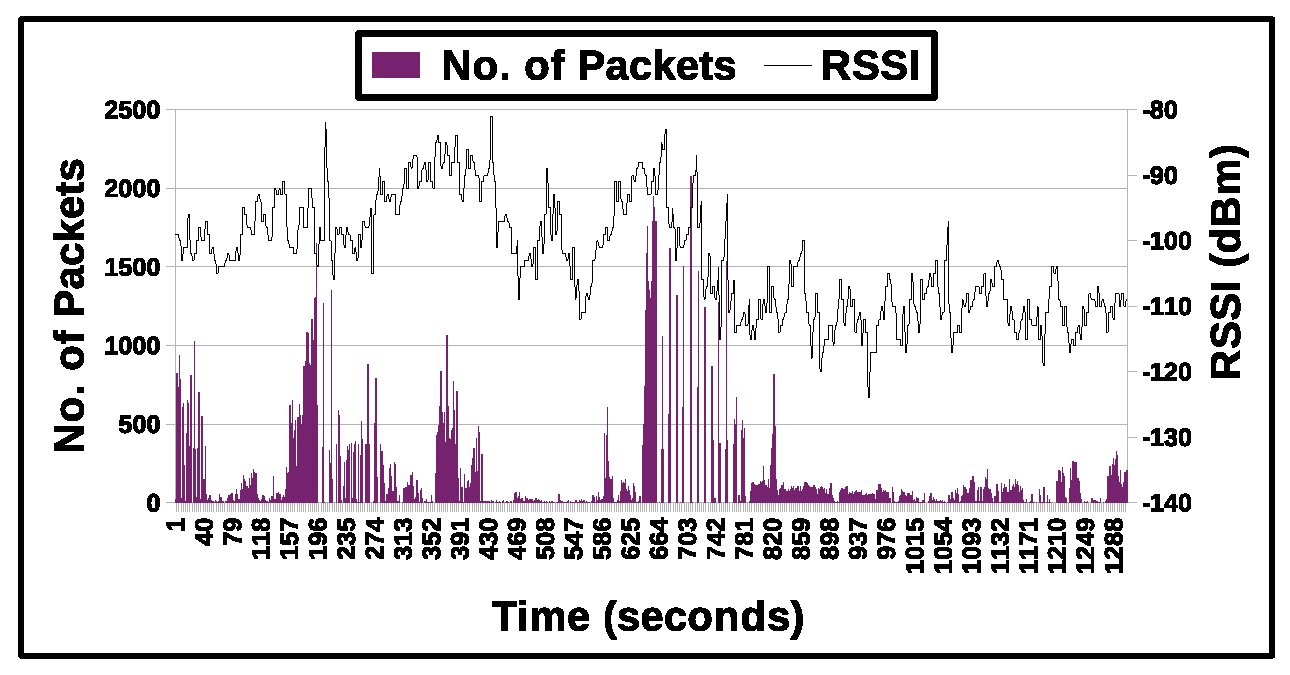
\includegraphics[width=0.4\textwidth,trim={0cm 0cm 0cm 1cm}]{figures/video_rssi_thrpt.eps}}%
%\caption{Experimental Observations}\vspace*{-0.5cm}
%\end{figure*}
A \textit{key finding} of this experiment is shown in Fig.~\ref{fig:chap04:technology_with_traj}, which displays the trajectory of a Moto G5 phone connected to the Airtel network on a single day over the IIT Kharagpur campus area of $8.5$ sq.km. It is seen that even within the small area covered, the phone connects to different generations of cellular technologies, each highlighted in different colours. Two inferences can readily be drawn from Fig. Fig.~\ref{fig:chap04:technology_with_traj}. (i) A service provider does not guarantee a complete \ac{4G} connectivity across the entire coverage region. A \ac{UE} often has to fallback to legacy \ac{3G} or \ac{2G} networks. (ii) Even when connected to \ac{4G}, the signal strength shows random variations. For example, for the experiments conducted, the \ac{RSSI} of \ac{4G} networks fluctuates between $-87$dBm to $-115$dBm. This portrays the typical connectivity scenario in many regions in India.
Another important observation from our experiments, shown in Fig.~\ref{fig:chap04:pcap_RSSI}, is that the volume of data downloaded by video players is not always commensurate with the current network signal strength. Several opportunities to download large chunks of data at high signal strength conditions remain unexploited.


\indent Video streaming applications, including live streaming, predominantly use \ac{DASH} \cite{stockhammer2011dynamic}. In this protocol, the target video is broken into chunks of fixed playback time, and multiple copies of each chunk is stored  at different quality levels, i.e., bitrates.  The client side video player uses \ac{ABR} algorithms~\cite{mao2017neural,Spiteri2016,yin2015control,Raca2019,Akhtar2018}
to decide on the  bitrate at which the next chunk is to be fetched. Existing \ac{DASH} algorithms  primarily take bitrate decisions based on the estimated network throughput or the playback buffer size while attempting to improve user's \ac{QoE}. We, on the other hand, hypothesize that it is possible to significantly lower the energy usage without sacrificing \ac{QoE} if we intelligently utilize the nuances of the cellular network throughput fluctuation during ABR streaming.


\indent To this end, we build an energy
efficient video player {\bf EnDASH} as a wrapper over \ac{DASH} (\S\ref{sec:chap04:sys_overview}).
EnDASH predicts the average cellular network throughput over a finite future time window to take decisions on the opportune fetching of video chunks by dynamically increasing the playback buffer size (\S\ref{sec:chap04:sys_overview}). So, it (i) predicts the the cellular network link throughput from radio related parameters (\S\ref{sec:chap04:thpre}), (ii) then uses the predicted throughput to predict the playback buffer length, and (iii) finally uses the predicted buffer length to choose optimal bitrates for future chunks. Thus, EnDASH consists of three prediction modules, of which the throughput prediction uses random forest learning (step (i)). However, EnDASH works over a smartphone connected to a cellular network which is a randomly varying environment. So, it uses Deep Reinforcement Learning (RL) for the buffer-length prediction mechanism (step (ii)) and bitrate adaptation (step (iii)), which allows EnDASH to exploit the actual performance of previous choices to tune its operation to the current characteristic of the network.  Consequently, EnDASH can start without any apriori knowledge and gradually learn through exploration and exploitation.  The playback buffer length and bitrate decision engines use Deep Neural Networks to map `raw' observations to outputs. These two engines operate using $A3C$ \cite{mao2017neural}, a state-of-the-art actor-critic RL algorithm, and run asynchronously with respect to one another. We train individual prediction modules over a large corpus of collected data traces and evaluate EnDASH using an emulation environment.


\indent Evaluation using our emulation platform shows that in comparison to existing \ac{ABR} algorithms~\cite{mao2017neural,Spiteri2016,yin2015control}, EnDASH significantly improves the energy savings in smartphones (\S\ref{sec:chap04:evaluation}). Energy saved from playing a $2200$ second video using EnDASH can be used to gain an additional $1440$ seconds of video playback time in comparison to the popular Pensieve algorithm~\cite{mao2017neural}. The energy savings, however, comes at the cost of marginally reduced \ac{QoE}.
One of the most salient features of EnDASH, which sets it apart from existing \ac{ABR} algorithms~\cite{mao2017neural,Spiteri2016,Sengupta2018,yin2015control,Raca2019,Akhtar2018,Schulman2010} is that its throughput prediction engine captures the impact of not only the received signal strength but also other network related parameters, such as different technologies and vertical handovers. 
The Mean Absolute Percentage Error (MAPE) of the throughput prediction engine of EnDASH varies from $8\%$ to $13\%$ across different scenarios. The improvement is particularly pronounced in regions having a substantial presence of legacy networks.
The improved throughput prediction assists the EnDASH RL engine to accurately capture the playback buffer evolution, which in turn aids the video segment download in an energy-efficient but QoE favourable manner.\vspace*{-0.2cm}

\section{\textbf{Background and Related Work}}\label{sec:chap04:related_work}
\indent \ac{4G} LTE smartphones are designed to maintain network connectivity using a \ac{RRC} state machine with two states: \textit{CONNECTED} and \textit{IDLE} \cite{Huang2012}. With no active transmission, the \ac{UE} is in the low power \ti{IDLE} state where no radio resource is assigned.  Once a packet arrives, the  \ac{UE} jumps to the high power \ti{CONNECTED} state, in which radio resources are assigned and data transmission takes place.  To reduce the incumbent delay and energy consumption associated with the state promotion, the \ac{UE} waits for a duration called tail time in the \ti{CONNECTED} state before returning to the \ti{IDLE} state even after packet transmission is over. To save energy in the tail period, LTE uses  \ac{DRX} during which the cellular interface periodically monitors the control channel for incoming packets and then goes to sleep ~\cite{Huang2012}. Evidently, if video is downloaded during poor connection quality, then the smartphone will have a longer \ti{CONNECTED} state dwell time resulting in higher energy consumption. Existing \ac{ABR} video streaming algorithms, however, primarily focus on improving \ac{QoE} while paying little attention to energy savings.


\noindent \textbf{Improving QoE:}
\ac{ABR} video streaming algorithms either choose buffer occupancy~\cite{Huang2014,Spiteri2016}  or both buffer occupancy and current chunk or network throughput~\cite{MPC-SIGCOMM-2015,Jiang2014,Sengupta2018,Xu2015,Mehr2019} to select optimal bitrates for future video chunks. Examples would be BOLA \cite{Spiteri2016} and MPC \cite{MPC-SIGCOMM-2015}, respectively.
Pensieve \cite{mao2017neural} uses a deep RL algorithm for optimal bitrate selection to maximize over a \ac{QoE} metric. However, none of these  works focus on saving device energy consumption under mobility conditions in \ac{4G} LTE networks. \\
\indent In this work, we aim to improve video user's energy consumption over cellular networks while not compromising on \ac{QoE} by tuning playback buffer size to network throughput. Hence, the proposed algorithm should use cellular network throughput prediction.
Several works focus on bandwidth prediction for improving the bitrate selection of  ABR streaming algorithms~\cite{Bentaleb2019,Raca2019,Raca2018_2,yue2018linkforecast}. Some of these works also focus on predicting cellular network throughput~\cite{Raca2019,yue2018linkforecast,Raca2017,Raca2018_2,Raca2018_3,Samba2017, Ghasemi2018}. However, unlike our EnDASH algorithm, none of the works consider the unique situation of co-existence of different technologies and frequent handover from one technology to another for throughput prediction.


\noindent\textbf{Reducing Energy Consumption:} Several works in literature investigate energy consumption reduction of mobile phones independently of QoE or ABR streaming algorithms. The BarTendr algorithm in \cite{Schulman2010}  tunes the download sessions in 3G networks to the network conditions for saving energy. However, it quantifies the network condition using received signal strength only while giving no weightage to handovers or associated technologies. GreenTube in \cite{Xin2012} proposes to tune cache management to user behaviour and network conditions. A popular method to reduce energy consumption in mobile phones is to optimize the tail energy, which is achieved in ~\cite{Yang2018} by either prefetching or delaying packets.

\indent To tune packet downloads to network conditions so as to save energy requires a detailed energy profiling of the phones and service providers. This can be obtained through detailed measurement studies as in \cite{Huang2012}. While~\cite{Zhang2018M,Zhang2016,Zhang2016DASH,Khokar2019} focus on the measurement of power consumption of video traffic over HTTP in \ac{4G} networks, the effect of  mobility on signal strength  in \ac{4G} networks is presented briefly. In~\cite{Huang2012, Deng2018} are presented  measurement studies on mobility support in \ac{4G} \ac{LTE} networks. However, to the best of our knowledge, there is no comprehensive measurement study on video streaming under mobility in cellular-only networks. Furthermore, an inherent assumption in these papers is the uninterrupted availability of 4G signal. In contrast, the present work focuses on optimization of energy consumption and \ac{QoE} of mobile video users in scenarios where legacy networks are present in addition to 4G, under mobility conditions.
\section{\textbf{Pilot Study}}\label{sec:chap04:motivation}
\begin{figure}[ht]
	\captionsetup[subfigure]{width=0.49\linewidth}
	\begin{center}
		\subfloat[\label{fig:chap04:setup}The Experimental Setup inside a slow moving electric vehicle]{
			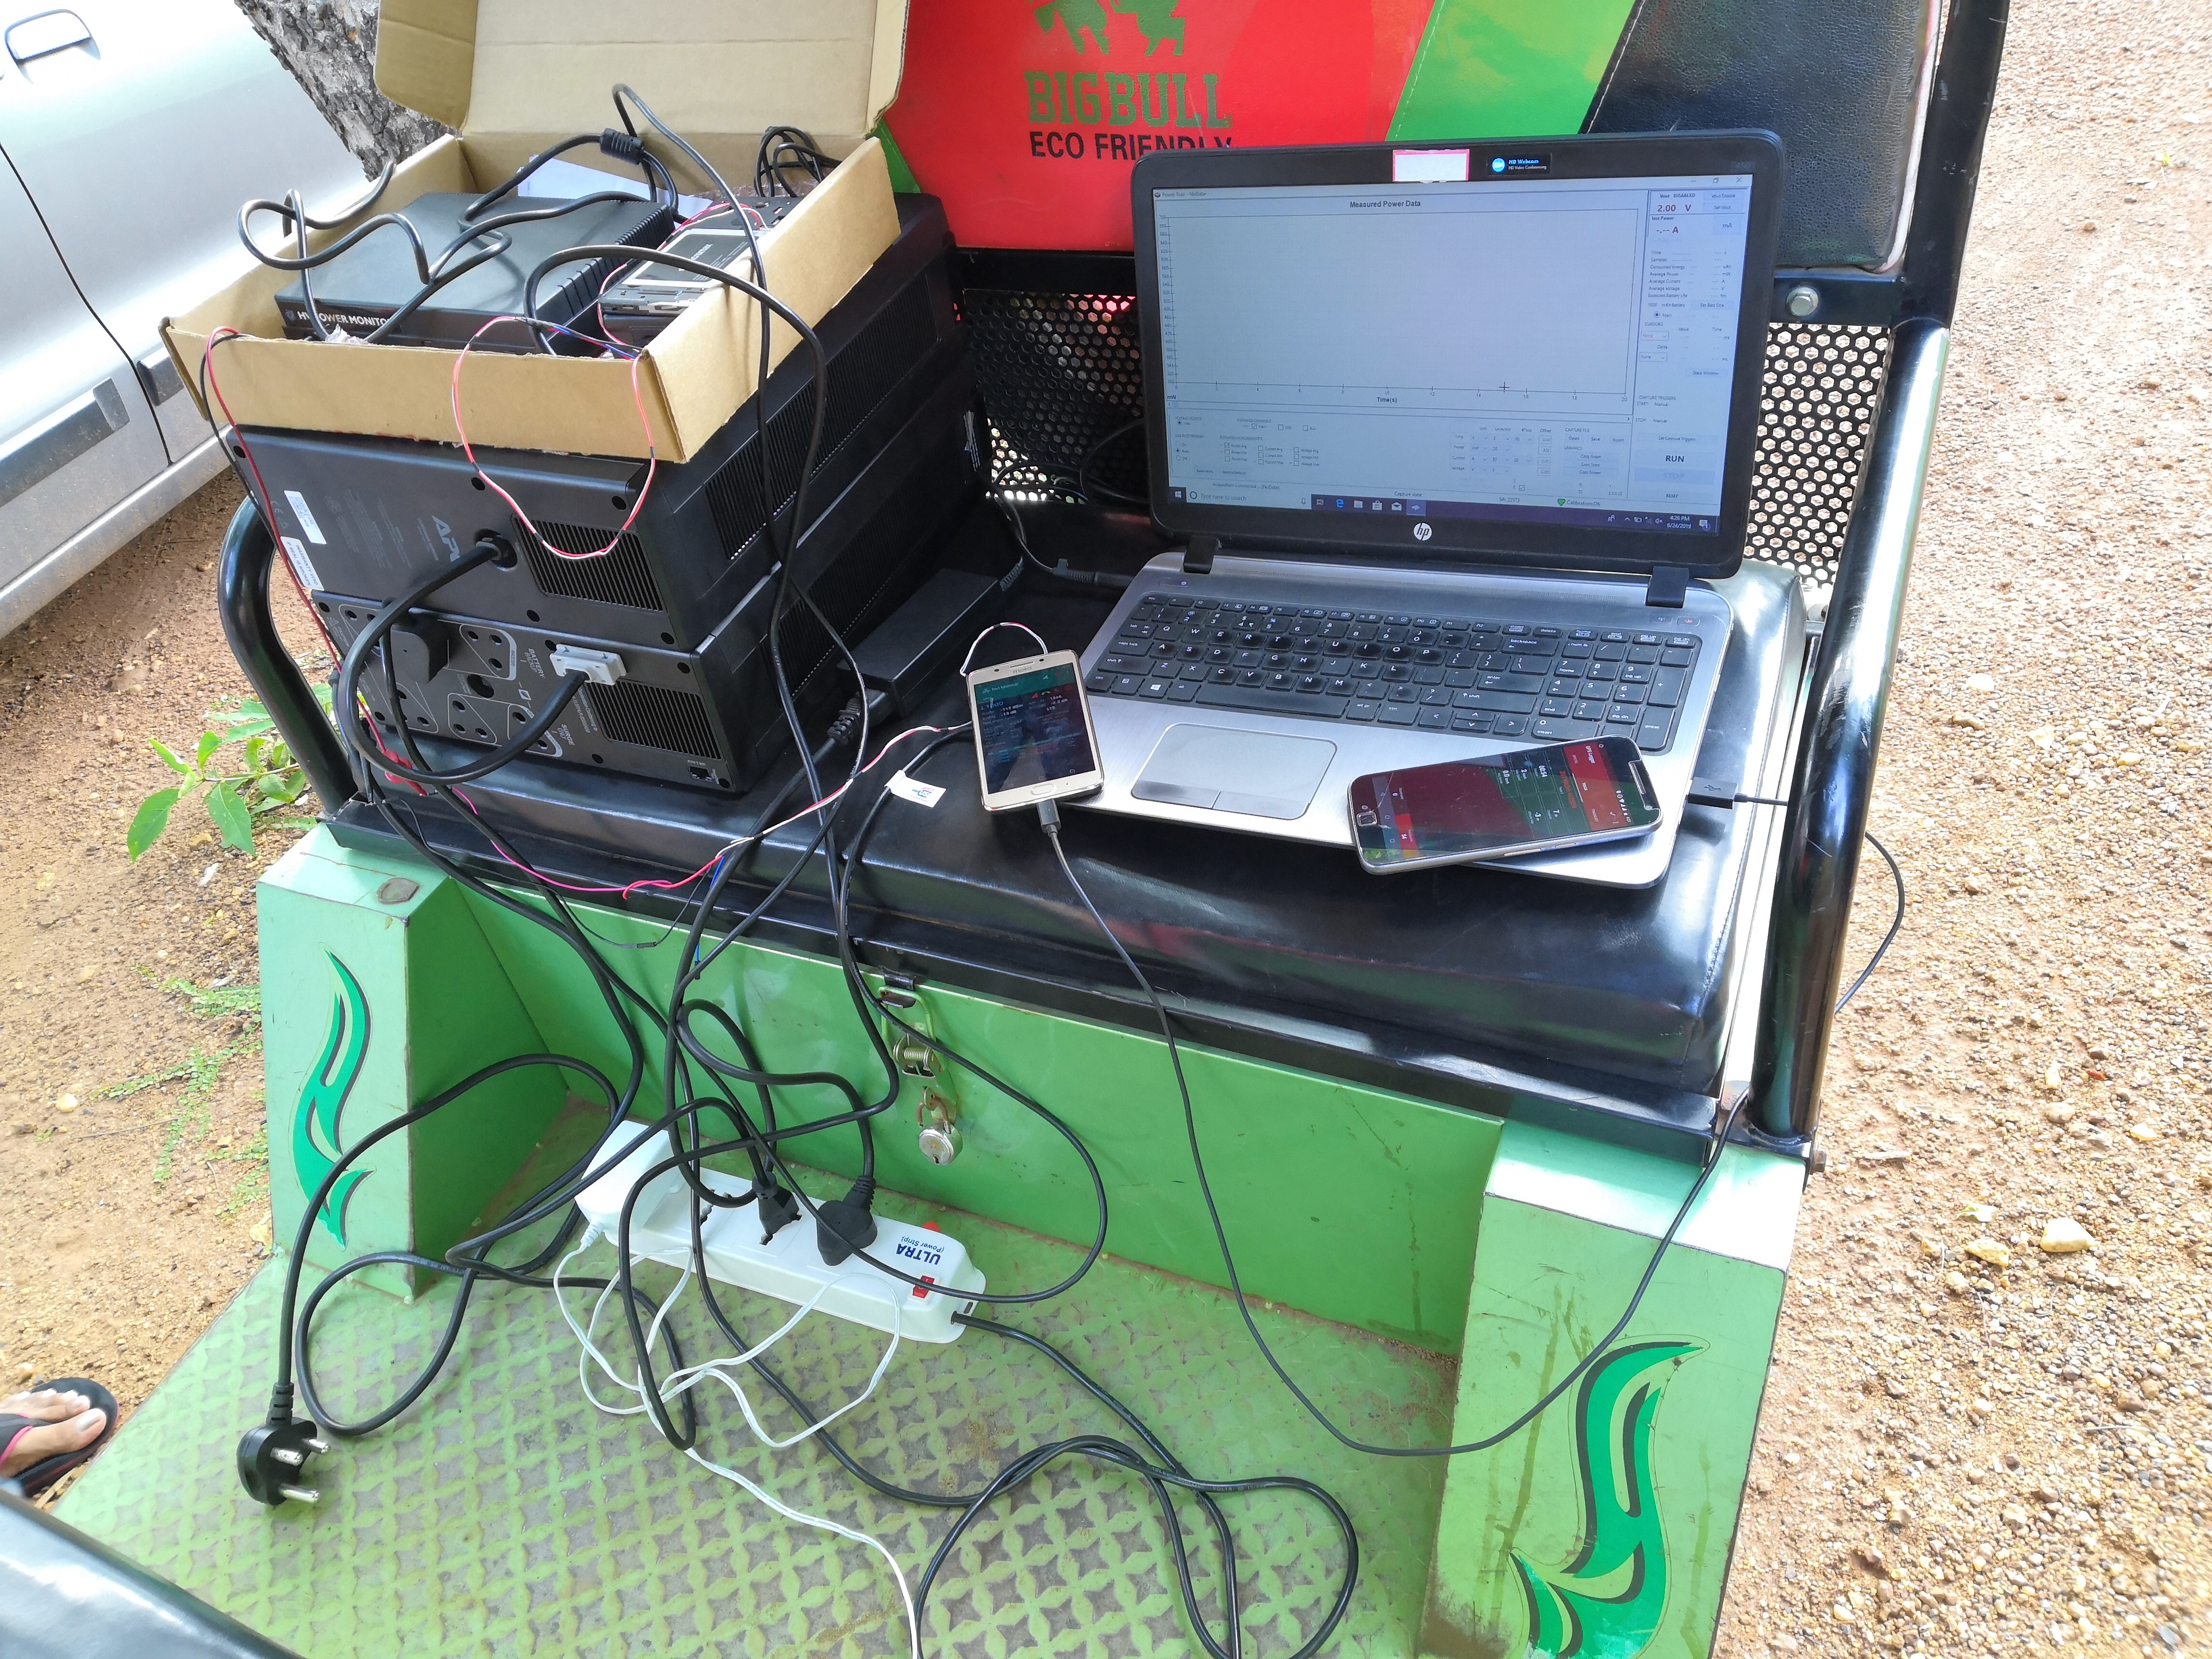
\includegraphics[width=0.49\linewidth]{figures/setup.png}
		}
		\subfloat[\label{fig:chap04:thptHO}Sorted throughput of the twenty-nine stretches of \fig{\ref{fig:chap04:technology_with_traj}} and its corresponding variations with RSSI, Vertical and Horizontal Handovers]{
			\fbox{\includegraphics[width=0.49\linewidth]{new_results/pilot/location_throughput}}
		}\\
		\subfloat[\label{fig:chap04:powerHO}Variations of Power Consumption with RSSI, and Vertical and Horizontal Handovers over the user's trajectory shown in \fig{\ref{fig:chap04:technology_with_traj}}]{
			\fbox{\includegraphics[width=0.49\linewidth]{new_results/pilot/location_power}}
		}
	\end{center}
	\caption{Experimental setup and Throughput and Power consumption variations of a user under mobility; Phone: Moto G5, Service Provider: Airtel}
\end{figure}
%\begin{figure*}[t]%
%\centering
%\subfigure[The Experimental Setup inside a slow moving electric vehicle]{%
% \label{fig:setup}%
% 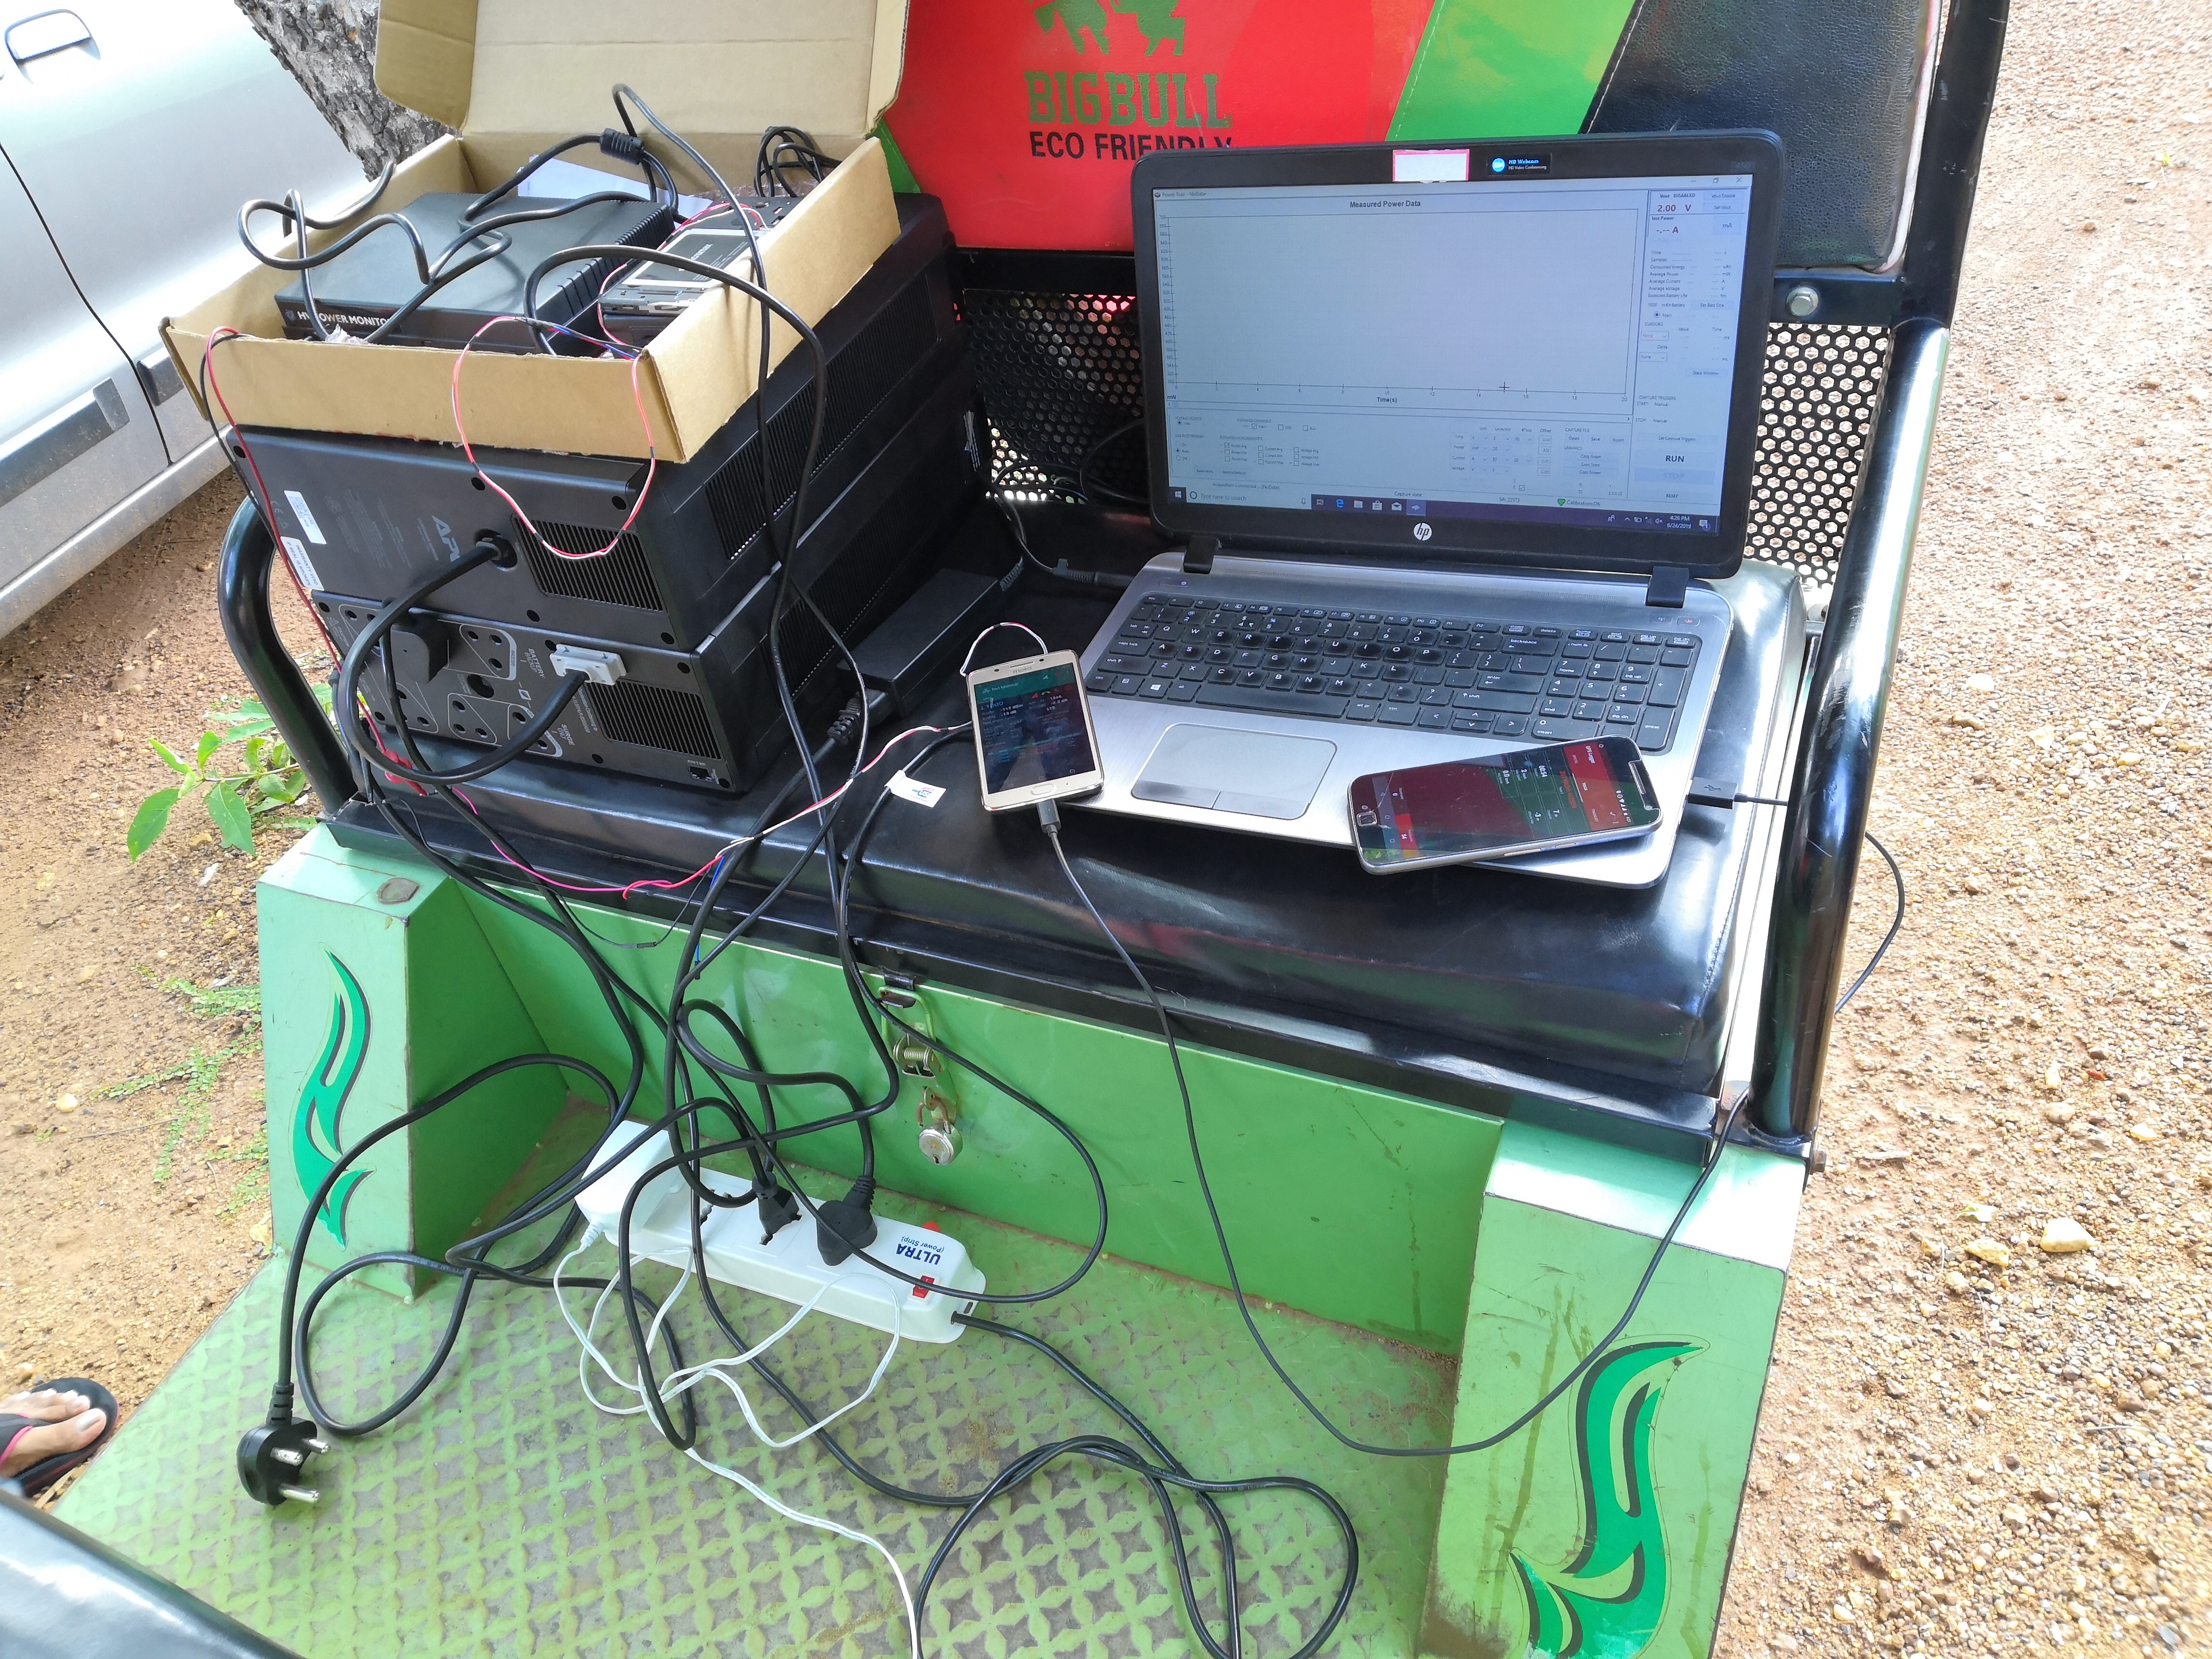
\includegraphics[width=0.31\textwidth]{figures/setup.png}}%
%\hspace{0.1cm}
%\subfigure[Sorted throughput of the twenty-nine stretches of \fig{\ref{fig:technology_with_traj}} and its corresponding variations with RSSI, Vertical and Horizontal Handovers]{%
% \label{fig:thptHO}%
% \fbox{\includegraphics[width=0.31\textwidth]{new_results/pilot/location_throughput}}}%
%\hspace{0.1cm}
%\subfigure[Variations of Power Consumption with RSSI, and Vertical and Horizontal Handovers over the user's trajectory shown in \fig{\ref{fig:technology_with_traj}}]{%
%\label{fig:powerHO}%
%\fbox{\includegraphics[width=0.31\textwidth]{new_results/pilot/location_power}}}
%\caption{Experimental setup and Throughput and Power consumption variations of a user under mobility; Phone: Moto G5, Service Provider: Airtel}\vspace*{-0.5cm}
%\end{figure*}
%\niloy{The context of the study is also not clear}
To design an energy efficient video streaming algorithm, which tunes playback buffer length with cellular network throughput, we need a detailed comprehension of the complex relationships between radio related parameters, such as signal strength, vertical and horizontal handovers, speed, etc., on one hand, and throughput and energy consumption on the other hand. To develop this understanding, we have carried out an extensive measurement based study as discussed next.
\subsection{Experimental Set-up}
\subsubsection{Hardware Setup}
For power consumption and energy profiling, we have selected medium budget VoLTE enabled smartphones -  Moto G5  (\$149) and Micromax Canvas Infinity (\$87). Table~\ref{tab:chap04:handset_details} outlines their configuration details. We record the power consumption of the phones using Monsoon Solutions High Voltage Power Monitor (HVPM) \cite{HVPM, Yang2018,Geng2015} (Fig.~\ref{fig:chap04:setup}) in both stationary and mobile conditions, when connected to three leading mobile internet service providers, Airtel, Reliance JIO, and Vodafone. The \ac{HVPM} records the power at a frequency of 5000 Hz. We have collected power consumption data in three different cities (Kolkata, Kharagpur, Guwahati).
\begin{table}[!t]
    \scriptsize
    \centering
      \caption{Details of the mobile handsets used}
    \begin{tabular}{|p{0.6cm}||p{3.4cm}|p{3.4cm}|}
    \hline
         \textbf{}  & \textbf{Moto G5 (Price: US\$ ~149)} & \textbf{Micromax Canvas Infinity (Price US\$ ~87)}\\
          \hline \hline 
         N/W Tech. & GSM/ HSPA/ LTE &  GSM/ HSPA/ LTE\\ \hline
         N/W Speed & HSPA 42.2/5.76 Mbps, LTE Cat4 150/50 Mbps & HSPA 42.2/5.76 Mbps, LTE Cat4 150/50 Mbps\\ \hline
         OS & Android 7.0 (Nougat) & Android 7.1.2 (Nougat) \\ \hline
         Chipset & Qualcomm MSM8937 Snapdragon 430 (28 nm) & Qualcomm MSM8917 Snapdragon 425 (28 nm)\\ \hline
         CPU & Octa-core 1.4 GHz Cortex-A53 & Quad-core 1.4 GHz Cortex-A53\\ \hline
         GPU & Adreno 505 & Adreno 308\\ \hline
    \end{tabular}
    \label{tab:chap04:handset_details}
\end{table}
\indent Besides power consumption, we have also collected extensive data on the received throughput of mobile phones in public buses, cars, and while walking across five cities of India (Kharagpur, Kolkata, Guwahati, Bengaluru, Malda). This dataset also includes data collected while travelling on highways. We have used workloads of 6Mb, 100Mb, 1GB file download, as well as of video streaming using Netflix, Hotstar, SonyLiv and Amazon Prime. This has allowed a detailed energy profiling of the smartphones. The entire corpus of collected data traces amounts to more than 50GB and has been collected over a period of eleven months. 
\subsubsection{Software Setup and Outcome}
\indent In this section, we outline the software setup. We have considered two primary workloads- (a) file download, and (b) video streaming. \\
\begin{figure}[h]
    \centering
    \fbox{\includegraphics[width=0.7\textwidth]{new_results/pilot/rssi_bin_time}}
    \caption{Total time spent in each \ac{RSSI} bin and the active time in each bin}
    \label{fig:chap04:vid_time}
\end{figure}
\begin{figure}[h]
    \centering
    \fbox{\includegraphics[width=0.7\textwidth]{new_results/pilot/rssi_bin_energy}}
    \caption{Amount of data downloaded \& Energy Consumption in \ac{RSSI} Bins}
    \label{fig:chap04:vid_thpt}
\end{figure}
% \begin{figure*}[t]%
% \centering
% \subfigure[Packet trace of a 360p Youtube video download with the temporal variation in the \ac{RSSI} during the download]{%
% \label{fig:pcap_RSSI}%
% 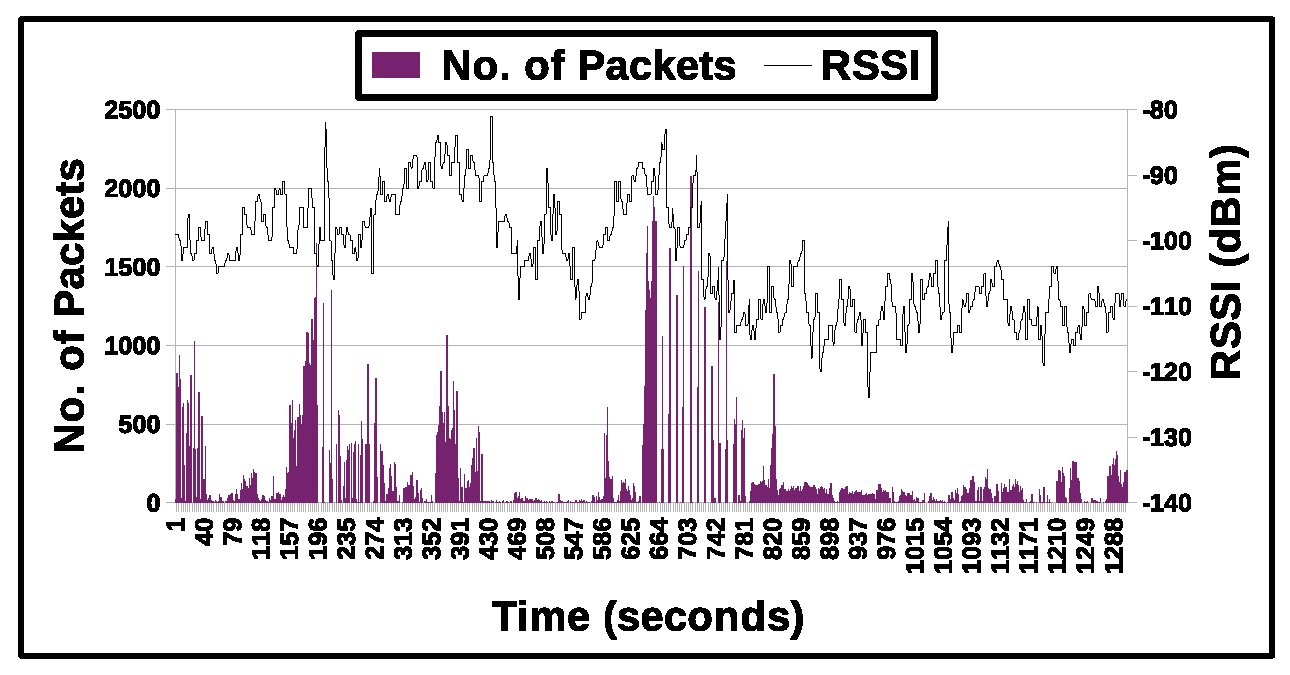
\includegraphics[width=0.31\textwidth]{figures/video_rssi_thrpt.eps}}%
% \hspace{0.1cm}
% \subfigure[Total time spent in each \ac{RSSI} bin and the active time in each bin]{%
% \label{fig:vid_time}%
% 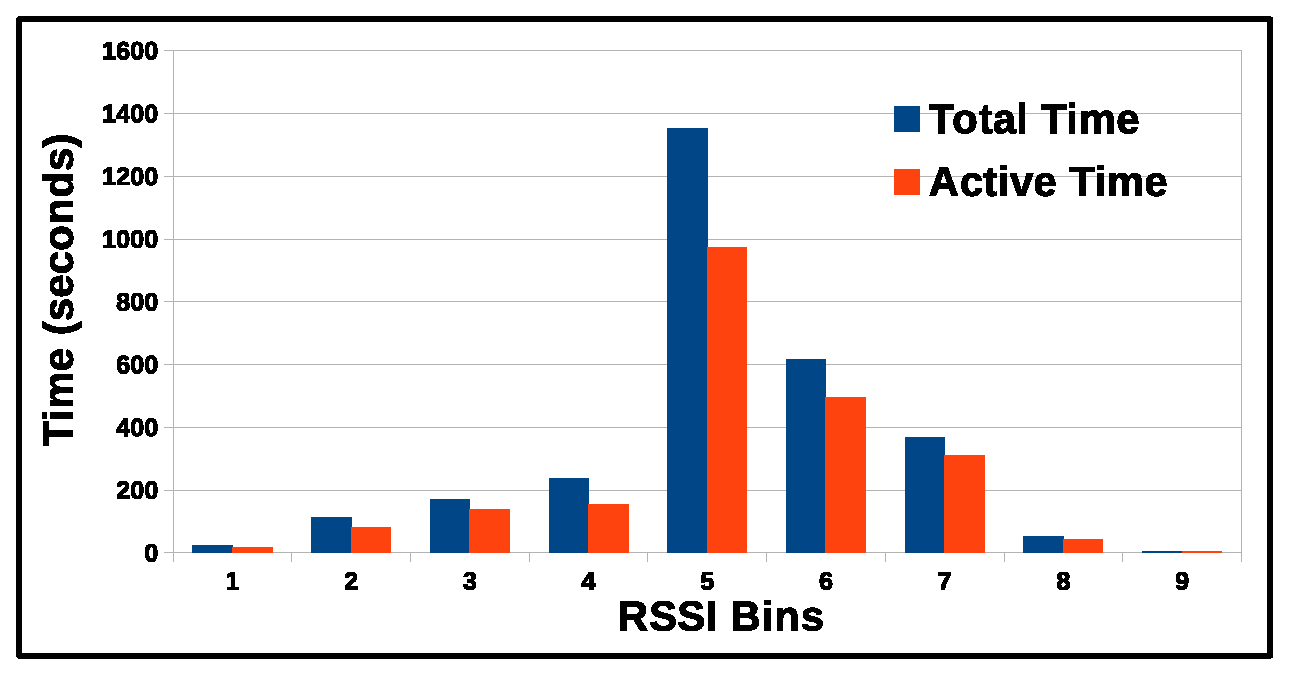
\includegraphics[width=0.31\textwidth]{figures/Video_Time_SNR_bins.eps}}%
% \hspace{0.1cm}
% \subfigure[Amount of data downloaded and Power Consumption in each \ac{RSSI} Bin]{%
% \label{fig:vid_thpt}%
% 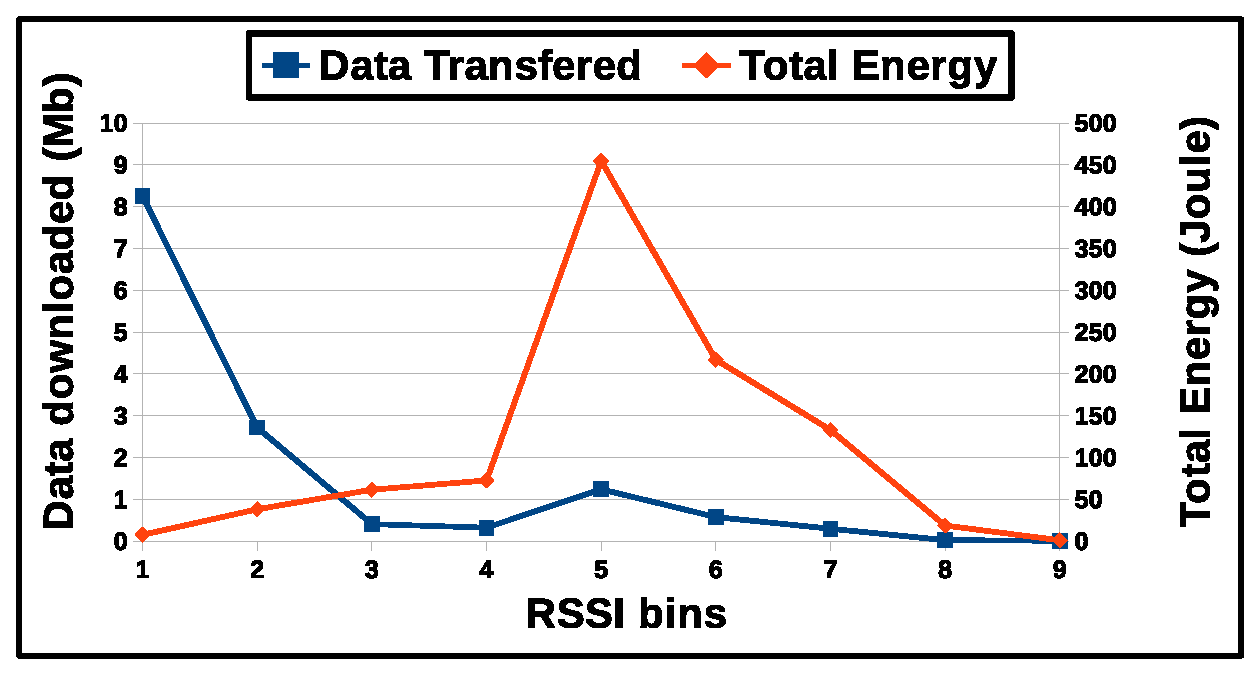
\includegraphics[width=0.31\textwidth]{figures/Video_thpt_power.eps}}%
% \caption{Statistics of YouTube video download to Moto G5 using Airtel mobile internet}\vspace*{-0.5cm}
% \end{figure*}
{\textbf{(a) File Download}} We have used file downloads to profile the power consumption in different RRC states. To enable the download, we have developed  an HTTP client-server program, where the client program runs in the phone and the server  is hosted on an Amazon Web Server (AWS). We have collected traffic traces, radio related information, and location and speed information using \ti{tcpdump}, Network Monitor Lite, and GPS Logger applications, respectively. The collected traffic traces have been analyzed using Wireshark. We have followed \cite{Yang2018} to derive  the RRC state diagram. Accordingly, to measure the \ti{IDLE} state power, we have kept the screen ON, uninstalled all non-default applications, kept all background applications disabled, the WiFi interface turned off, and the mobile network interface switched on but without any active traffic transmission. The corresponding power consumed by the operating system, processor, display, some default background and network-related operations, etc., constitutes the \ti{IDLE} state power.  We have continued measuring the power consumption starting from the \ti{IDLE} state, throughout the file download till the trace came back to the \ti{IDLE} power. Once a file download starts, a jump in power consumption is noted. After the download completes, it drops to an intermediate value during the tail time before returning to the \ti{IDLE} state \cite{Yang2018}. To derive the RRC states, we have downloaded files of different lengths several times using different phones and service providers  in the different cities in stationary condition. The power consumption and dwell time of each RRC state has been found to be different for different phones, service providers as well as c


\indent  Since the corpus of collected data traces is large, we use one such trace to discuss some interesting observations due to space limitations. We call this a `\ti{typical}' trace which was obtained on a single day when downloading 6MB files to the Moto G5 phone while moving around the IIT Kharagpur campus in a hybrid electric vehicle. The set-up is shown in Fig.~\ref{fig:chap04:setup}. As Airtel has significantly fluctuating signal quality inside the campus, we chose it as our service provider.  For this `\ti{typical}' trace we had downloaded a 6Mb file to our phone several times. During each download session, the vehicle had moved over a different stretch of the trajectory inside the IIT Kharagpur campus.  Of all the downloads, the twenty-nine stretches  shown in \fig{\ref{fig:chap04:technology_with_traj}} could be identified as valid. The sorted throughput over all the twenty-nine stretches of  \fig{\ref{fig:chap04:technology_with_traj}} is plotted in descending order in \fig{\ref{fig:chap04:thptHO}}. The $x$-axis represents the location indices corresponding to the sorted throughput. The mean and variance of the \ac{RSSI} and also the horizontal and vertical handovers in each of these stretches is shown in \fig{\ref{fig:chap04:thptHO}}.  It is observed that the throughput is affected more negatively by handovers than \ac{RSSI} fluctuations. For example, the average and the variance of \ac{RSSI} is nearly the same  in location stretches-\textbf{29} and \textbf{15}. However, stretch \textbf{29} has a lower throughput due to handovers. Again, vertical handovers between network technologies  are found to have a more negative impact on throughput than horizontal ones, as seen in location stretches {\bf 22}  and {\bf 4}.  The effect of handovers on the variation of \ti{CONNECTED}, \ti{TAIL} and \ti{IDLE} state power is shown in Fig.~\ref{fig:chap04:powerHO}. It is seen that stretches that witness handovers have a higher variance in  power consumption than no handover stretches. This is because, during handovers, there is a high amount of control information exchange which leads to the rise in \ti{IDLE} power. Moreover, handovers are associated with lower throughput which increases the \ti{CONNECTED} power. Fluctuating signal quality during handover increases the retransmissions and hence the TAIL state power variations.


$\mathrm{\mathbf{\underline{Takeaway:1}}}:$ \textit{The wireless network condition is best quantified by throughput which depends  significantly on phenomena such as handovers and not  on received signal quality alone.}\\
{\textbf{(b)Video Streaming}}\label{sec:chap04:vstreaming}
To understand how throughput fluctuation affects video streaming, 
we show the packet trace of a YouTube video of length 20 minutes captured when moving along the trajectory of \fig{\ref{fig:chap04:technology_with_traj}}.  Although we learn from the previous section that it is best to quantify the network condition using throughput, in this section we analyze the video download using \ac{RSSI} only. This is because it is difficult to capture the actual network throughput of a phone while any other application (in this case YouTube) is running.\\
\indent The  captured trace and the \ac{RSSI}  is shown in \fig{\ref{fig:chap04:pcap_RSSI}}. It is seen that the application downloads video chunks even at low \acp{RSSI}. To understand this, we have divided the \acp{RSSI} on the secondary $y$-axis of \fig{\ref{fig:chap04:pcap_RSSI}} into nine bins each of width five, starting from -81 dBm to -126 dBm. The time the \ac{UE} spends in each of these bins, and the time it remains active is given in \fig{\ref{fig:chap04:vid_time}}. It is seen that the percentage of time the \ac{UE} spends in the best \ac{RSSI} bin, i.e. \bin{1} (-85 to -81 dBm) is less than 1\%. In comparison, the highest dwell time   as well as the highest active time is recorded in \bin{5} where the \ac{RSSI} varies between -115 to -111 dBm. If we focus on the energy consumption in these \ac{RSSI} bins, as given in \fig{\ref{fig:chap04:vid_thpt}}, it is seen that the highest energy is also consumed by the phone in \ac{RSSI} \bin{5}. Another obvious effect of downloading at low signal strength is the low amount of data downloaded for a longer amount time; with reference to \ac{RSSI} \bin{5} in \fig{\ref{fig:chap04:vid_thpt}}.


\indent The rate at which the YouTube playback buffer is filled depends on: a) the bandwidth available, and b) the quality of the video requested by the user. Once the buffer length exceeds a threshold, the download stops and restarts only when the buffer length goes below the threshold. So, if the buffer is full when signal quality improves, then the phone does not download any video packet - a possible explanation for no data download between  430-547 seconds in \fig{ \ref{fig:chap04:pcap_RSSI}}.


$\mathrm{\mathbf{\underline{Takeaway:2}}}:$ \textit{The current protocol of  video download attributes a higher weightage to the playback-buffer length than the user's instantaneous received signal strength or throughput, ensuing a significantly high energy consumption.}\\
\indent The takeaways of the pilot study provide the design criteria for designing the EnDASH system, discussed next. 
\section{\textbf{EnDASH System}}\label{sec:chap04:sys_overview}
The proposed EnDASH system is an energy efficient client video player, working as a wrapper over \ac{DASH}. It predicts the cellular network throughput over a finite future time window to take decisions on the opportune fetching of  video chunks.  EnDASH operates in a time-slotted fashion. So, the entire timeline is divided into discrete time-slots of length \mq{T}.
EnDASH executes the following functions to achieve energy efficient video download: (i) At the beginning of each time slot it uses historical data on radio parameters to predict the cellular network link throughput of the current time slot using a Random Forest Learning (RFL) engine. (ii) It then uses the predicted throughput to predict the optimal playback-buffer length for the current slot that minimizes energy consumption. For this, EnDASH employs the state-of-the-art \ac{A3C} deep \ac{RL} algorithm.  (iii) Before downloading each video chunk within a time slot, EnDASH runs another A3C based deep \ac{RL} engine to predict the optimal download chunk  bitrate. 
EnDASH is, thus, a cascaded system of three engines: (i) throughput prediction, (ii) buffer length decision,  and (iii) bitrate selection as shown in Fig.~\ref{fig:chap04:EnDASH system}. We next describe these modules.
 \begin{figure}[t]
	\centering
	\includegraphics[width = 0.7\textwidth,trim = {1cm 1cm 1cm 1cm}]{figures/EnDASH_system.pdf}
	\caption{Composite Representation of the EnDASH model; a cascaded model where the predicted throughput acts as an input network state to the Actor Critic \ac{RL} based decision engine}
	\label{fig:chap04:EnDASH system}
\end{figure}
 \subsection{The Throughput Prediction Engine}\label{sec:chap04:thpre}
EnDASH employs a \ac{RFL} algorithm for cellular network throughput prediction ~\cite{Raca2019}. At the beginning of time slot \mq{t}, it uses the historical information of different radio related parameters in the previous \mq{x} seconds to predict the average throughput~\footnote{Since video rate adaptation algorithms mostly use average throughput, hence for EnDASH, we have predicted the average throughput only \cite{Raca2019}.} that may be experienced by the user during the time slot (of length `T'). We represent this as $\prefu{x}{T}$.
The input features of the throughput prediction engine are: (i) \ti{RSSI}, (b) \ti{technologies used} - LTE (4G), HSPA+ (3.75G), UMTS (3G), EDGE (2G), (c) \ti{number of vertical and horizontal \ti{handovers}}, (d) \ti{speed},  (e) \ti{number and technology of neighbouring \acp{BS}}, (f) \ti{download link throughput} - the download rate is measured at the \ac{UE} in bytes per second. Readings on these features  are obtained from the NetMonitor Lite app with a granularity of one second.

\indent  Each feature can be represented as a distribution,
However, instead of feeding the entire time-series data for each metric, we adopt the summarization technique of \cite{Raca2019}. So, we feed only a few key values that best summarize the data and its corresponding distribution.
For each of the features we obtain the $\mathrm{25^{th}}$, $\mathrm{75^{th}}$, and $\mathrm{90^{th}}$ percentile points, median and mean from its historical data and feed it to the \ac{RFL} algorithm. We train and test this module using 39662 seconds of collected data on received throughput across five Indian cities.
 
\subsection{The Buffer Length Decision Engine}\label{sec:chap04:buff_length_dec_engine}
\indent The Buffer Length Decision engine also runs at the beginning of each time slot and the playback buffer length is predicted from the predicted network throughput.  However, the relationship between the predicted throughput and the buffer length is not straightforward and is not analytically tractable. So, we employ an A3C \ac{RL} based deep neural network to determine the optimal buffer length.
 
\indent The components of the \ac{RL} algorithm corresponding to the buffer decision engine are as follows:\\
% \begin{itemize}
\noindent \textbf{(i) Environment}  \ti{E} - video player.\\
\noindent \textbf{(ii) Input state at timeslot \mq{t}} $S_t$ =  ($\hat{\tau}_{{t}}$, $B_{av_t}$, ${\mathcal{X}}$), where
  $\hat{\tau}_{{t}}$ is the  average predicted cellular network throughput,
 $B_{av_t}$ is the current playback buffer capacity available in seconds,
$\mathcal{X}$ is the set of possible changes in buffer length. If the current buffer length is $B_{t-1}$, the next buffer length can be predicted to be $\hat{B_t}= B_t+x$ where $x\in\mathcal{X}:=\{-2,-1,0,+1,+2\}$. $x=1$ implies an increase in buffer length by a single chunk, each chunk is of eight seconds.\\
\noindent \textbf{(iii) Action} $A_t$ - Decisions on the increase or decrease of buffer length at timeslot $t$. \\
\noindent \textbf{(iv) Reward} - The reward function is defined as a linear weighted function of energy savings with respect to a baseline ABR algorithm and the QoE score:
    \begin{equation}
    \Xi_{\mathrm{bufflen}} = w_1 \cdot (\left|E_{\mathrm{EnDASH}_t}-E_{\mathrm{old}_t}\right|)+w_2 \cdot QoE
    \end{equation}

\indent The first term in the reward function gives the energy savings with respect to a baseline ABR algorithm. In this work, we have chosen BOLA \cite{Spiteri2016} as the baseline since its energy consumption is the lowest among existing algorithms (excluding EnDASH, \S{\ref{sec:chap04:evaluation}}).  $E_{\mathrm{old}_t}$ and $E_{\mathrm{EnDASH}_t}$ represent the energy consumption of BOLA and of EnDASH at time \mq{t}, respectively. The energy consumed while using one particular algorithm is obtained as follows:  the RRC states are first identified from the download packet capture of a video trace. Next, the dwell time in each RRC state is multiplied by the corresponding power consumption (obtained from the RRC state machine) to get the energy quantities. We calculate the energy savings in this manner because the ground truth on energy consumption cannot be obtained.

\indent Second term in the reward function is the \textbf{\ac{QoE}} metric  \cite{yin2015control}:
\begin{equation}\label{eq:chap04:QoE}
   \text{QoE} = \sum_{i=1}^N q(R_i) - \mu\sum_{i=1}^N \delta_i - \sum_{i=1}^{N-1}\left|q(R_{i+1})-q(R_i)\right|
\end{equation}
The $\text{QoE}$ metric is defined for a video with N chunks. $R_i$ is the bitrate of $\text{chunk}_i$ and $q(R_i)$ maps the bitrate to a quantity which represents the quality perceived by the user. We have taken $q(R_i) = R_i$ \cite{mao2017neural}. $\delta_i$ is the rebuffering time involved in downloading $\text{chunk}_i$ at bitrate $R_i$. $\mu$ represents the degree of penalty associated with $\delta_i$.  We have taken $\mu=4.3$ \cite{mao2017neural}. The last term represents the playback smoothness. The QoE decreases when there is abrupt variability in throughput between successive chunks. Thus, QoE increases with bitrate, and reduces with rebuffering time and throughput variability.
\subsection{The Bitrate Decision Engine}
 \label{sec:chap04:bitrate_dec_engine} 
The predicted playback buffer length is next used for selecting optimal chunk bitrates using a deep \ac{RL} based algorithm. The components of the \ac{RL} algorithm are:\\

\noindent\textbf{(i) Environment}  \ti{E} - video player.\\
\noindent\textbf{(ii) Input state before downloading the chunk \mq{n}}, \\$S_{n}$ = ($\hat{\mathcal{B}_t}, \tau_c(n-1)$, $d_{n-1}$, $l_{n-1}$, $B_{n}$, $\zeta_{n}$, $r_{n}$), where $\hat{\mathcal{B}_t}$- predicted playback buffer length for current slot \mq{t}, $\tau_c(n-1)$= throughput of last chunk, $d_{n-1}$ = time taken to download last chunk, $l_{n-1}$ = bitrate of last chunk, $B_{n}$ = available playback buffer length, $\zeta_{n}\in\bracket{s_1,s_2,\cdots s_m}$ = Possible size of next video chunk  ($m$ available sizes), $r_{n+1}\in \bracket{R_1, R_2,\cdots, R_6}$ = Possible bitrate levels for next video chunk.\\
\noindent\textbf{(iii) Action} $A_n$ - Optimal bitrate decision for the next chunk.\\ 
\noindent\textbf{(iv) Reward}- QoE score obtained from Eqn.~(\ref{eq:chap04:QoE}).\\
\indent The buffer length and bitrate decision engines run at two different time scales. So, time slot indices for the variables related to the buffer length decision engine and the bitrate decision engine are denoted by  \mq{t} and \mq{n}, respectively.
\subsection{Emulation environment for \ac{RL} training}
In the training phase, the \ac{RL} agent of the buffer and the bitrate decision engine of EnDASH should ideally be trained using real video downloads at actual video streaming clients. 
However, this demands that entire chunks be downloaded for each training data point. Further, downloads over cellular networks can be quite slow. Hence, to save training time, we train EnDASH and its competing  ABR algorithms using an emulation environment that closely mimics a real video client application. The emulator maintains its own representation of a real client's playback buffer. At the beginning of a time slot, the emulator first predicts the average throughput and then the playback-buffer length for the slot. Within the slot, once a chunk is to be downloaded, the emulator first assigns a download time to the chunk based  on its bitrate and the internal network throughput, derived from previous chunks. It then depletes the playback-buffer by the chunk's download time to emulate the playback-buffer drainage during an ongoing chunk download. It adds the playback duration of the  chunk being currently downloaded to the playback-buffer. The emulator sleeps temporarily once the playback buffer is full. Rebuffering occurs if the playback-buffer is completely drained before the next chunk download. The emulator keeps track of the rebuffering event and rebuffering time. After each slot (chunk download), the emulator prepares the state $S_t$ ($S_n$) for the \ac{RL} module of the buffer decision (bitrate decision) engines.
\subsection{The \ac{RL} Training algorithm}
Both the buffer length and bitrate decision engines of EnDASH are trained using  state-of-the-art actor-critic method, which involves training two neural networks \cite{mao2017neural}: an actor network and a critic network. A3C is a policy gradient \ac{RL} algorithm which estimates the gradient of the total reward from the trajectories of the execution followed by a policy. The action is chosen based on the policy by the actor network while the critic network estimates the advantage of selecting the action by returning a value function. Both networks update their weights in each time step.
 
\indent Each parameter of the state \ti{S} of both buffer length and bitrate decision engines are passed on to their respective actor and critic network to enable learning of optimal buffer lengths and bitrates by the corresponding \ac{RL} modules~\cite{mao2017neural}.
As in \cite{mao2017neural}, we initiate multiple learning agents to accelerate the training. By default, there are 16 agents. Each agent is designed to experience a different set of input parameters, e.g., network traces. However, the learning agents continuously report  their individual tuples of (state, action, reward)  to a central model, which aggregates them to generate a single model.
\subsection{Implementation of the \ac{RL} modules}
\begin{figure}[ht]
	\captionsetup[subfigure]{width=0.49\linewidth}
	\begin{center}
		\subfloat[\label{fig:chap04:EnDASH_en}Energy Consumption]{
			\includegraphics[width=0.33\textwidth]{new_results/simres/Energy}
		}
		\subfloat[\label{fig:chap04:EnDASH_QoE}QoE score (Eqn.~\ref{eq:chap04:QoE})]{
			\includegraphics[width=0.33\textwidth]{new_results/simres/QoE}
		}
		\subfloat[\label{fig:chap04:EnDASH_buff}CDF of buffer length]{
			\includegraphics[width=0.33\textwidth]{new_results/simres/BuffOccu}
		}
	\end{center}
	\caption{\label{fig:chap04:EnDASH_vs_others}Performance comparison of EnDASH with baseline \ac{ABR} streaming algorithms, BOLA \cite{Spiteri2016}, Pensieve \cite{mao2017neural}, Fast MPC \cite{yin2015control}, Robust MPC \cite{yin2015control}}
\end{figure}
%  \begin{figure*}[t]%
%  	\centering
%  	\subfigure[Energy Consumption]{%
%  		\label{fig:EnDASH_en}%
%  		\includegraphics[width=0.33\textwidth]{new_results/simres/Energy}}%
%  	\subfigure[QoE score (\ref{eq:QoE})]{%
%  		\label{fig:EnDASH_QoE}%
%  		\includegraphics[width=0.33\textwidth]{new_results/simres/QoE}}%
%  	\subfigure[CDF of buffer length]{%
%  		\label{fig:EnDASH_buff}%
%  		\includegraphics[width=0.33\textwidth]{new_results/simres/BuffOccu}}
%  	%\hspace{0.1cm}
%  	\caption{Performance comparison of EnDASH with baseline \ac{ABR} streaming algorithms, BOLA \cite{Spiteri2016}, Pensieve \cite{mao2017neural}, Fast MPC \cite{yin2015control}, Robust MPC \cite{yin2015control}}
%  	\label{fig:EnDASH_vs_others}
%  \end{figure*}
\begin{figure}[ht]
	\captionsetup[subfigure]{width=0.49\linewidth}
	\begin{center}
		\subfloat[\label{fig:chap04:avg_bitrate}Avg. Bitrates in Mbps]{
			\includegraphics[width=0.49\linewidth]{new_results/simres/AvgBitrate}
		}
		\subfloat[\label{fig:chap04:stall}Stall Time per segment (in seconds))]{
			\includegraphics[width=0.49\linewidth]{new_results/simres/Stall}
		}\\
		\subfloat[\label{fig:chap04:smooth}Bitrate Variation]{
			\includegraphics[width=0.49\linewidth]{new_results/simres/BitrateVar}
		}
	\end{center}
	\caption{\label{fig:chap04:indi_QoE}Comparison of different components of \ac{QoE} score (average bitrate, stall time, smoothness) of EnDASH with baseline \ac{ABR} streaming algorithms, BOLA \cite{Spiteri2016}, Pensieve \cite{mao2017neural}, Fast MPC \cite{yin2015control}, Robust MPC \cite{yin2015control}}
\end{figure}
%  \begin{figure*}[t]%
%  	\centering
%  	\vspace*{-0.5cm}
%  	%\hspace{0.1cm}
%  	\subfigure[Avg. Bitrates in Mbps]{%
%  		\label{fig:avg_bitrate}%
%  		\includegraphics[width=0.33\textwidth]{new_results/simres/AvgBitrate}}%
%  	%\hspace{0.1cm}
%  	\subfigure[Stall Time per segment (in seconds)]{%
%  		\label{fig:stall}%
%  		\includegraphics[width=0.33\textwidth]{new_results/simres/Stall}}%
%  	\subfigure[Bitrate Variation]{%
%  		\label{fig:smooth}%
%  		\includegraphics[width=0.31\textwidth]{new_results/simres/BitrateVar}}%
%  	\caption{Comparison of different components of \ac{QoE} score (average bitrate, stall time, smoothness) of EnDASH with baseline \ac{ABR} streaming algorithms, BOLA \cite{Spiteri2016}, Pensieve \cite{mao2017neural}, Fast MPC \cite{yin2015control}, Robust MPC \cite{yin2015control}}\vspace*{-0.5cm}
%  	\label{fig:indi_QoE}
%  \end{figure*}
The \textit{bitrate selection engine} of EnDASH is adopted from the state-of-the-art Pensieve algorithm \cite{mao2017neural}, which also uses A3C to learn optimal bitrates. We have used a pretrained model provided by Pensieve, albeit with different input states.  The \textit{buffer length decision engine} has been implemented in Tensorflow \cite{Abadi2016}. The engine passes five previous values of the buffer length to a 1D convolution layer (CNN) with 128 filters, each of size 4 with stride 1. The remaining inputs, i.e., predicted link throughput and current available buffer length are passed onto another 1D-CNN having the same shape. Results obtained from these layers are subsequently combined in a hidden layer having 128 neurons and uses the softmax function. The same inputs are also used by the critic network, which has the same neural network, but whose final output is a linear neuron. During the training of the algorithm, we set the discount factor to 0.9, i.e., current actions are allowed to be influenced by 100 future steps. The learning rates for the actor and the critic networks are 0.0001 and 0.001, respectively. The entropy factor $\beta$ has been set to gradually decrease from 1 to 0.1 over iterations.

\section{\textbf{Evaluation}}\label{section:evaluation}

In this section we evaluate EnDASH and compare its performance with other popular \ac{ABR} algorithms, in terms of \ac{QoE} and energy consumption. We first discuss the methodology that we have adopted.
\subsection{Methodology}
% There are three decision engines in the EnDASH system- (i) the throughput prediction engine, (ii) the buffer length decision engine, (iii) bitrate selection engine. These engines are inividually trained before being integrated together. 
%\subsubsection{Data Traces}
To train and test the throughput engine of EnDASH, we have used a corpus of throughput and power consumption traces collected under user mobility, for both file download and video streaming workloads. These include data collected using Moto G5 and Micromax Canvas Infinity phones over Airtel, Reliance JIO, and Vodafone networks, across five cities in India. The entire corpus is of 39662 seconds of data. The real-life throughput traces are formatted to be compatible with the Mahimahi \cite{Netravali2015} network emulation tool. We have divided the collected data set into 70-30 ratio for training and testing. To train the RL algorithms of the buffer length and bitrate decision engine, we have used another  dataset of 57 DASH-ified videos having a total duration of 45 hours. 
The baseline \ac{ABR} streaming algorithms that we have used are \ti{BOLA} \cite{Spiteri2016}, \textit{Pensieve}\cite{mao2017neural}, \textit{Fast MPC} \cite{Yin2015}, and \textit{Robust MPC} \cite{Yin2015}. 
%These algorithms have been discussed in \S\ref{section:lit}.
%\subsubsection{Baseline ABR algorithms}
% \niloy{Are these adaptive streaming algorithm}
% \begin{itemize}
%     \item \textbf{BOLA:} Using Lyapunov optimization, BOLA \cite{Spiteri2016} selects bitrates for future video chunks considering only the playback buffer occupancy status.
%     \item \textbf{Pensieve:} It uses a actor critic reinforcement learning algorithm to maximize over a QoE metric \cite{mao2017neural}.
%     \item \textbf{Fast MPC:} FastMPC \cite{Yin2015} uses buffer occupancy and past throughput to optimize \ac{QoE} metric for next five chunks.
%     \item \textbf{Robust MPC:} Robust MPC \cite{Yin2015} further improves FastMPC by accounting for the predicted and actual throughput of the last five chunks.
% \end{itemize}
% \subsubsection{Quality of Experience (QoE) metric}
% Different users show different choices when watching videos. For example, while some may prefer a very high quality, others may want reduced rebuffering/stall time. Yet others may want a less fluctuating video quality or a minimum startup time. It is widely accepted that a higher rebuffering time often emerges as the strongest cause of dissatisfaction among users. Considering all these factors, the \ac{QoE} metric commonly used by most existing works is \cite{Yin2015}:
% \begin{equation}\label{eq:QoE}
%   \text{QoE} = \sum_{i=1}^N q(R_i) - \mu\sum_{i=1}^N T_i - \sum_{i=1}^{N-1}\left|q(R_{i+1})-q(R_i)\right|
% \end{equation}
% The $\text{QoE}$ metric is defined for a video with N chunks. $R_i$ is the bitrate of $\text{chunk}_i$ and $q(R_i)$ maps the bitrate to a quantity which represents the quality perceived by the user. $T_i$ is the rebuffering time involved in downloading $\text{chunk}_i$ at bitrate $R_i$. $\mu$ represents the penalty associated with the rebuffering time. Higher is the value of $\mu$, heavier is the penalty. The last term represents the playback smoothness, and diminishes the QoE when there is abrupt variability in throughput between successive chunks. So, essentially, QoE increases with bitrate, and reduces with rebuffering time and throughput variability.\\
% \subsubsection{Reward function}
%\subsection{Results}In this section, we evaluate our proposed system EnDASH. First, we compare the performance of EnDASH with other baseline \ac{ABR} algorithms. We also show how a user benefits from using the EnDASH engine. Then, we present a microbenchmarking of the throughput prediction engine since its accuracy significantly affects the performance of EnDASH. 
\subsection{EnDASH versus Baseline ABR algorithms}
Fig. \ref{fig:EnDASH_vs_others} shows the energy consumption, \ac{QoE} score, and buffer length variation of EnDASH and other baseline \ac{ABR} algorithms. For evaluating these algorithms, the length of each time slot is set to $T=30$ seconds, and the length of the historical window is also set to $x=30$ seconds, i.e., $\prefu{30}{30}$. %So, the average throughput for a prediction window of 30 seconds is predicted using the historical data of 30 seconds. 
In existing literature, the Pensieve \cite{mao2017neural} algorithm has been reported to generate optimal chunk bitrates and video quality. Fig. \ref{fig:EnDASH_en} shows that EnDASH outperforms Pensieve in terms of energy consumption. However, this energy savings comes at the cost of sacrificing the \ac{QoE} with respect to Pensieve as seen in Fig. \ref{fig:EnDASH_QoE}. Moreover, while the average QoE of EnDASH is comparable with the other algorithms, the inter-quartile range of \ac{QoE} is significantly high, implying that the corresponding variability is high.  
 \subsection{QoE Performance Analysis}
To understand the \ac{QoE} performance in detail, we plot the individual components of the \ac{QoE} metric in \fig{\ref{fig:indi_QoE}}. We observe that the mean of the average bitrate (Fig. \ref{fig:avg_bitrate}) of EnDASH is smaller and its stall time (Fig. \ref{fig:stall}) is comparable with other algorithms. However, the mean bitrate variation (Fig. \ref{fig:smooth}) is much higher. Simultaneously, stall time displays a high variability. The reason for the reduced average bitrate, higher stall time variability, and higher mean of bitrate variation can be attributed to the tuning of the buffer length to the average throughput instead of the instantaneous throughput. For example, if the average throughput predicted is low, the system is forced to download a video chunk at a low bitrate for the entire timeslot, even though the throughput at multiple instances within the timeslot may be high, resulting in lower bitrates. Although the tuning to instantaneous throughput may improve bitrates, it will be associated with higher overhead. Hence, we focus on tuning to average throughput only. Further, the reduced inter-quartile range of the average bitrate is due to the aggressive fetching of video chunks. 
\subsection{Energy Performance Analysis}
EnDASH consumes much less energy because the video chunk download, and hence the playback buffer length, is tuned to the average predicted cellular network throughput. As a result, during high throughput conditions, the playback buffer length will increase, thereby facilitating the download of a higher number of chunks in a slot. This consecutive fetching of chunks reduces the tail energy which eventually manifests in the reduction of overall energy consumption as seen in Fig. \ref{fig:EnDASH_en}. The resulting trade-off is reflected in the increase in buffer length in comparison with the buffer length of competing ABR algorithms.  Fig. \ref{fig:EnDASH_buff} shows the CDF of playback buffer length of different algorithms. It is seen that while the maximum buffer length of existing algorithms is 50 seconds that of EnDASH can go up to 200 seconds; but this is a rare instance. In nearly 60\% of the time the buffer length remains below 50 seconds.
%\begin{figure}[ht]%
%\centering
%\subfigure[Energy Consumption and Extra Playtime obtained w.r.t. Fast MPC, which has the highest energy consumption]{%
%\label{fig:vid_time_save}%
%\includegraphics[width=0.23\textwidth]{new_results/simres/EnergyConsumption}}%
%\hspace{0.1cm}
%\subfigure[Energy Consumption of algorithms when watching videos of different lengths]{%
%\label{fig:energy_vid_length}%
%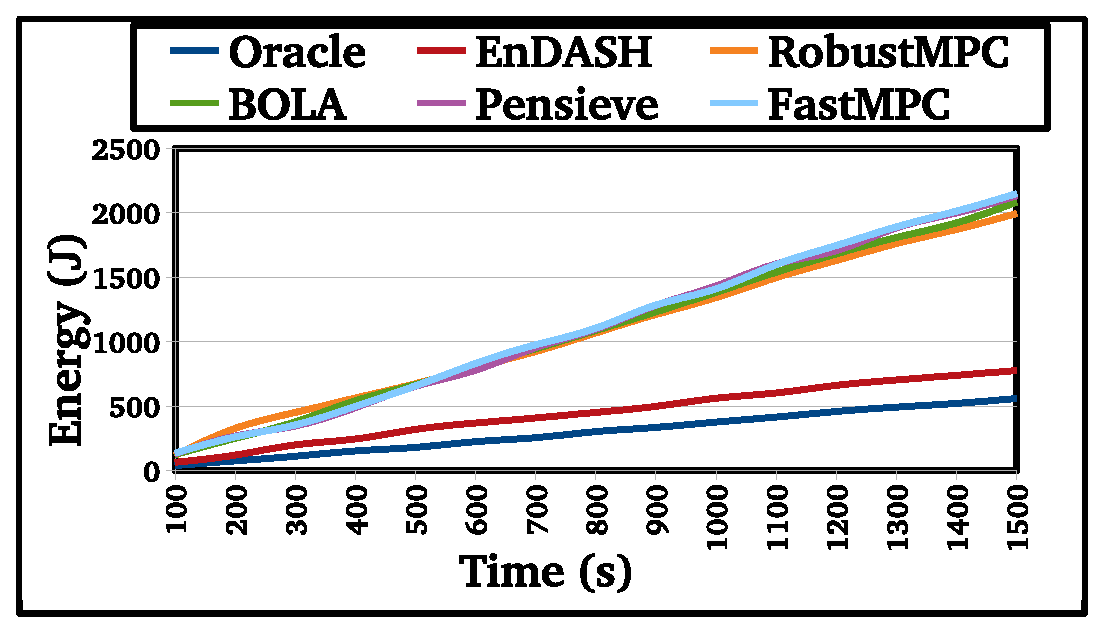
\includegraphics[width=0.23\textwidth]{figures/vid_length_energy.eps}}%
%\caption{Comparison of the Energy Performance of EnDASH with baseline \ac{ABR} streaming algorithms}\vspace*{-0.5cm}
%\label{fig:energyperf}
%\end{figure}
\begin{figure}[ht]%
	\centering
	{\fbox{\includegraphics[width=0.7\linewidth]{new_results/simres/EnergyConsumption}}}	
	\caption{Energy Consumption and Extra Playtime obtained w.r.t. Fast MPC, which has the highest energy consumption}
	\label{fig:vid_time_save}
\end{figure}
\subsection{Gain from Energy Savings}
\indent In this section, we discuss the gain in video playback time achieved by using EnDASH. FastMPC has the highest energy consumption among all algorithms. \fig{\ref{fig:vid_time_save}} shows the gain in video playback time achieved by the algorithms with respect to FastMPC while streaming a 2200 second video. It shows that using the energy saved by streaming the video using EnDASH, one can gain an additional 1403 seconds and 1440 seconds of video playback time in comparison with BOLA and Pensieve, respectively. Thus, one may infer that EnDASH can be used as a potential ABR streaming algorithm for increasing battery backup in smartphones.
%\indent Thus, our EnDASH algorithm offers a significant energy savings in conjunction with a reasonably high \ac{QoE}. The performance of EnDASH, however, depends heavily on the throughput prediction engine, various aspects of which are discussed next. 
\subsection{Feature importance study on throughput prediction engine} The primary objective of the throughput prediction engine is to account for the impact of cellular network technology change, i.e., the switching between 2G, 3G, 4G, etc., on network throughput.
\fig{\ref{fig:feature_imp}} shows the feature importance of different input parameters when predicting throughput. We observe that vertical handovers and associated technology (Network Type) have the highest weightage among all parameters, 0.32 and 0.21, respectively. The importance of such features in throughput prediction points out to
the absolute necessity of considering the existence of legacy systems when designing algorithms for 4G networks. 

\begin{figure}[!ht]
    \centering
    \includegraphics[width=0.7\linewidth]{new_results/simres/FeatureImpotance}
    \caption{Feature importance of the input parameters; signal strength, associated technology, and handovers (HOs)) between technology are the three features having the highest contribution in deciding throughput}
    \label{fig:feature_imp}
\end{figure}

\begin{figure*}[t]%
\centering
\subfigure[MAPE score measuring error of throughput prediction in different regions for various combinations of considering  associated technology and vertical handover (HO); for $\prefu{30}{30}$]{%
\label{fig:MAPE_diff_scene}%
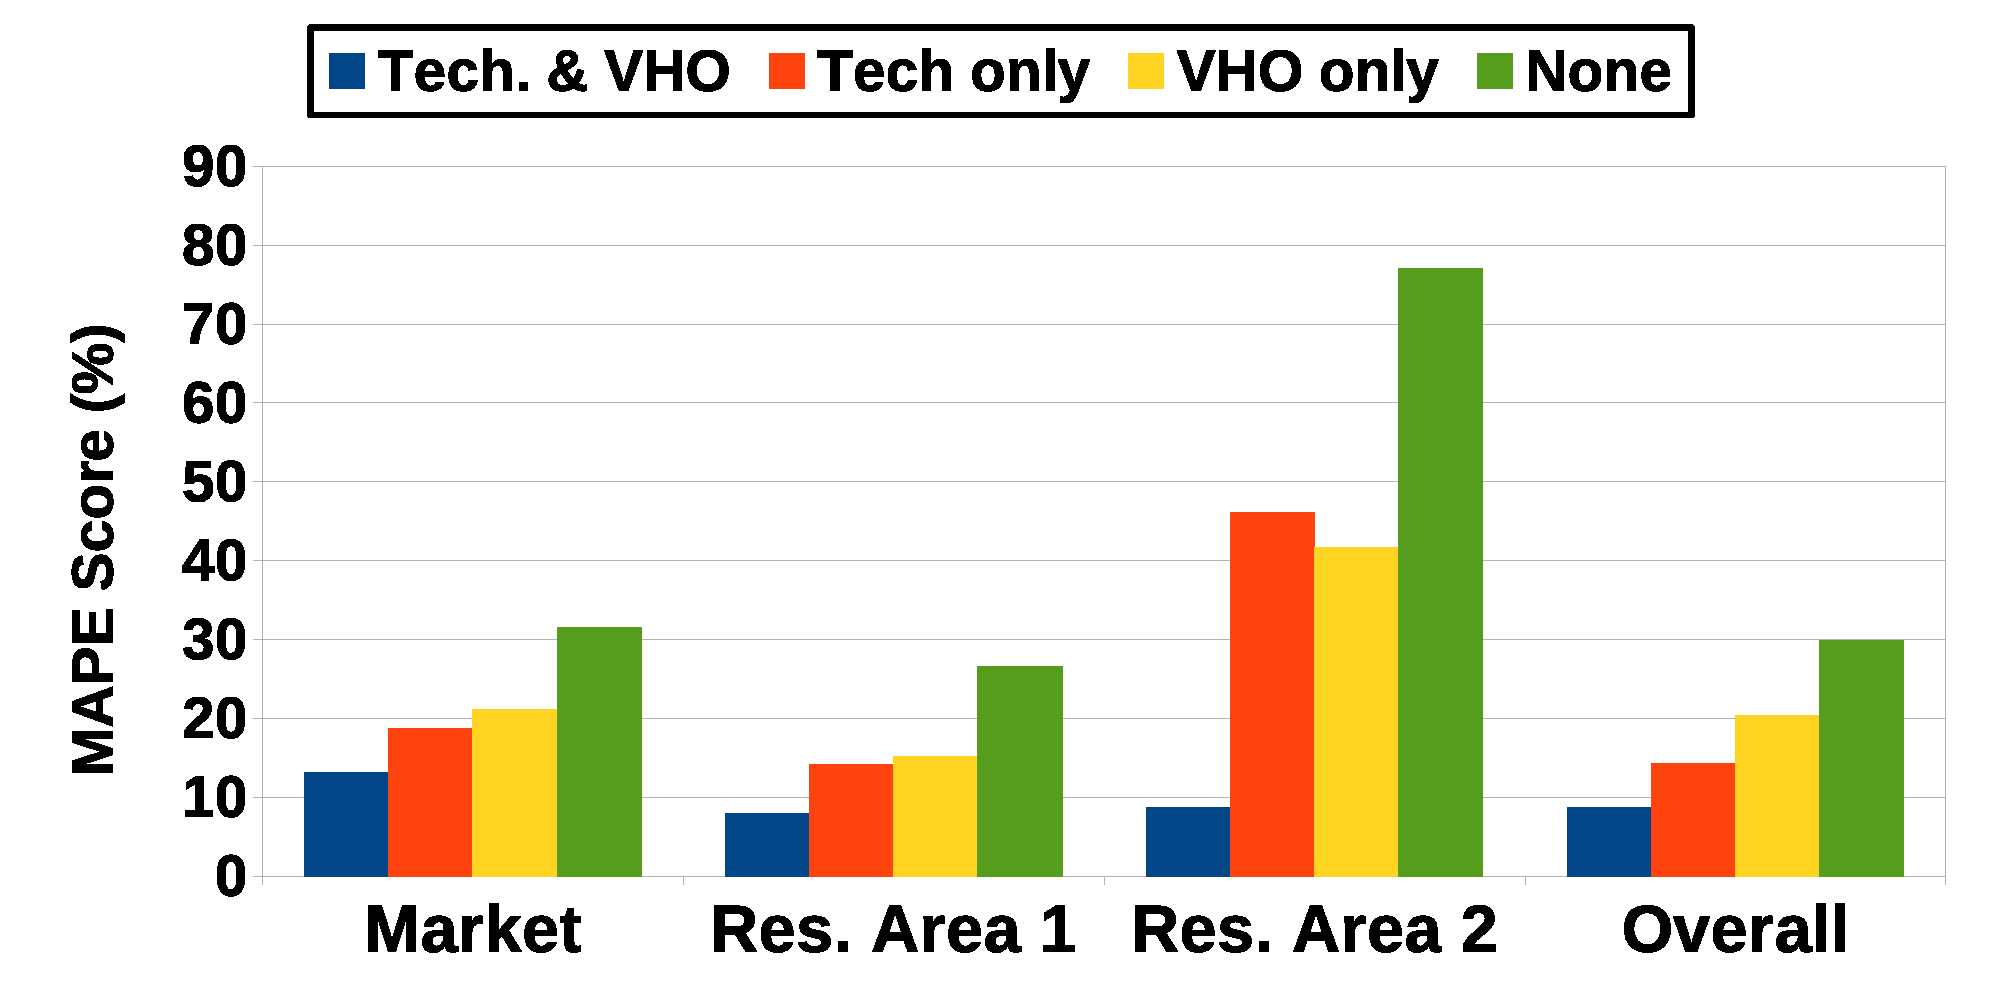
\includegraphics[width=0.48\textwidth]{figures/resi_vs_market_vs_overall_MAPE.eps}}
\hspace{0.02\textwidth}%
\subfigure[Impact of considering associated technology and vertical handovers (HOs) on performance metrics of EnDASH; for $\prefu{30}{30}$]{%
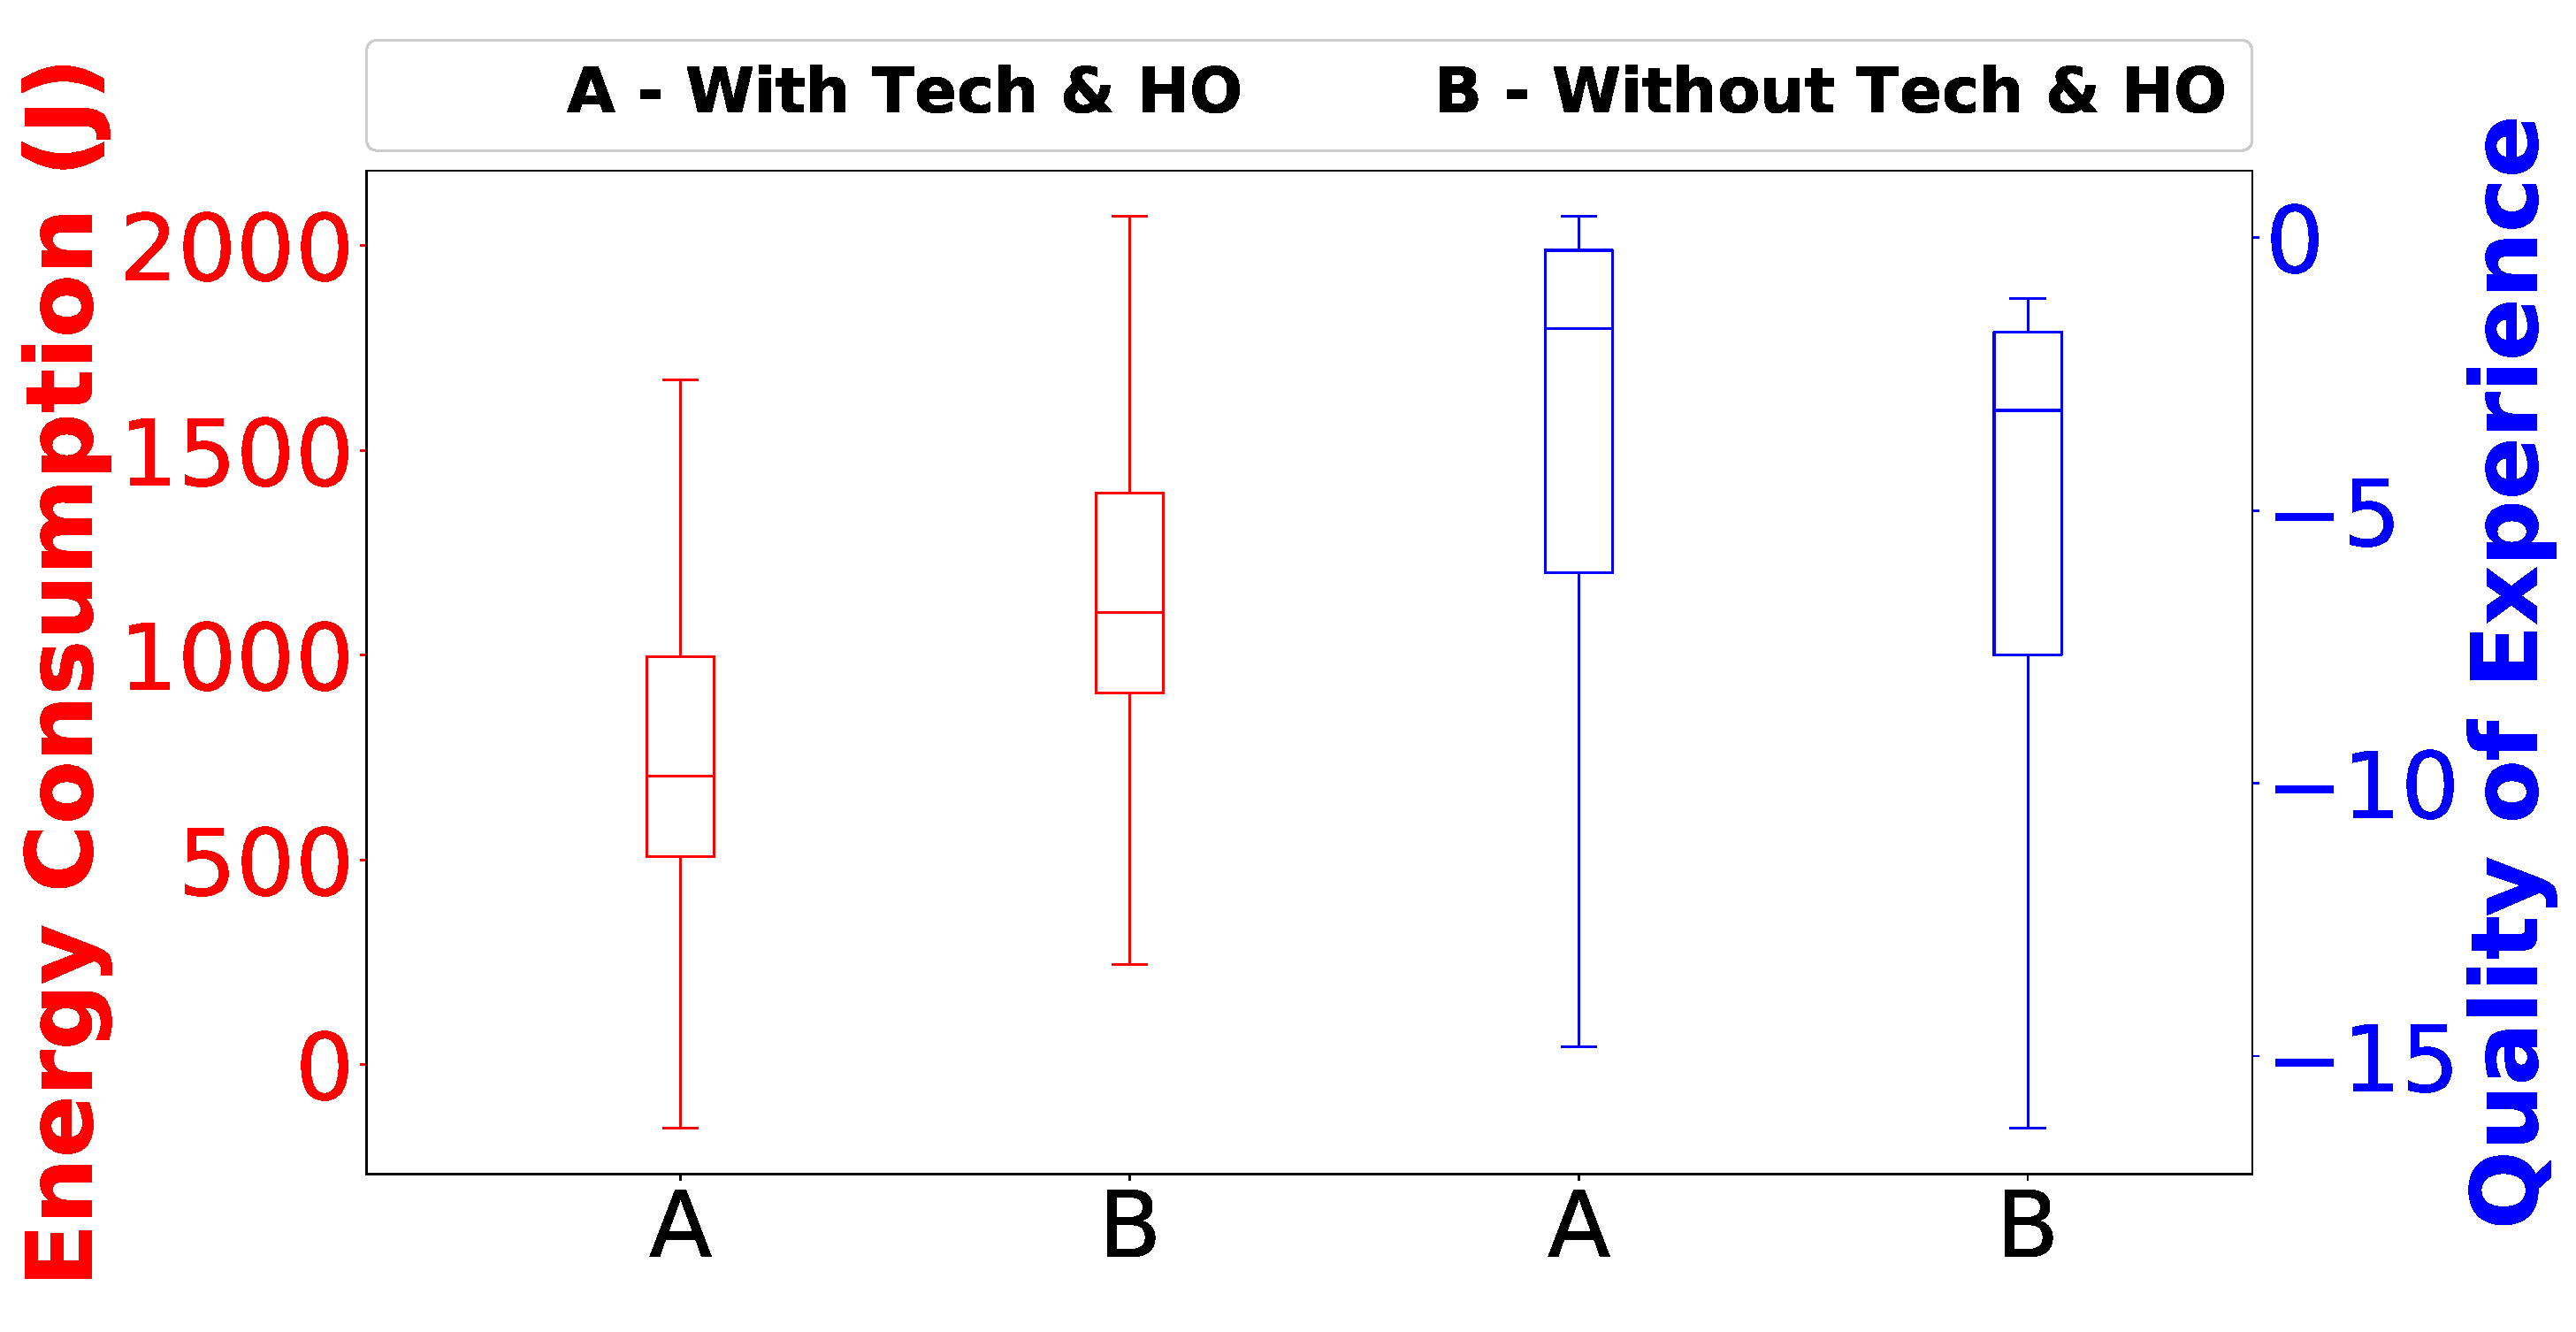
\includegraphics[width=0.48\textwidth]{figures/pow_qoe_comp.eps}}%

\subfigure[Predicted vs Actual throughput using the RF algorithm when associated technology and vertical handover (HO) is considered.]{%
\label{fig:thpt_pred_trace}%
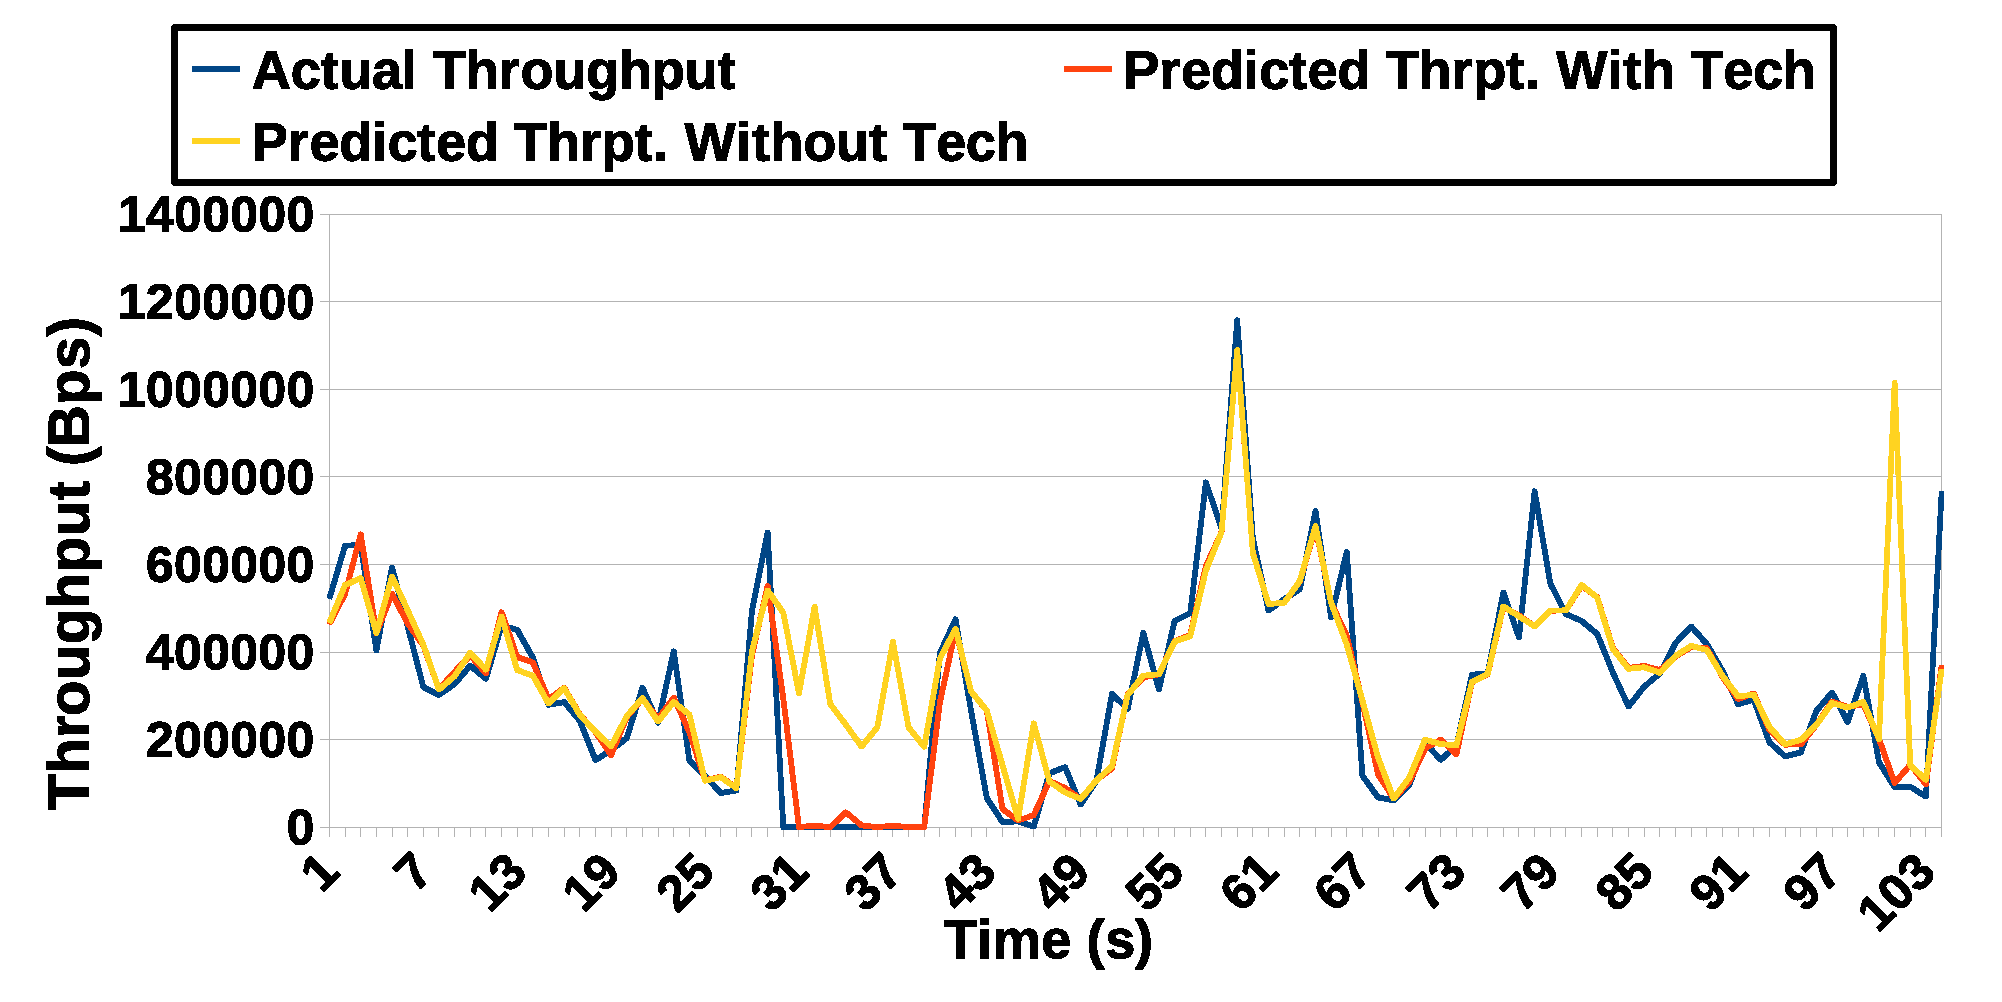
\includegraphics[width=0.49\textwidth]{figures/predicted_vs_actual_vs_Tech.eps}}%
\caption{Effect of Associated Technology and Vertical Handovers (HOs) on Throughput Prediction and EnDASH performance for $\prefu{30}{30}$}
\end{figure*}

\subsection{Importance of Associated Technology}
\indent To understand the impact of associated technology and vertical handovers on the throughput prediction error, we have evaluated the MAPE~\footnote{\indent MAPE score, which quantifies error in throughput prediction,  is:
\begin{align}
\text{MAPE\ score} = \frac{1}{N}\sum_{i=1}^N\left|\frac{\tau_i-\hat{\tau}_i}{\tau_i}\right|\times 100\%
\end{align}
where $\tau_i$ and $\hat{\tau}_i$ respectively denote actual and  predicted throughput in the $\mathrm{i^{th}}$ timeslot.} score over different regions. For this, we have divided the data traces collected in Kharagpur into three categories - (a) crowded Market Place, (b) a residential area with extensive 4G coverage (Residential Area 1), and (c) a residential area with limited 4G coverage (Residential Area 2). The overall MAPE score and the MAPE score for the three different scenarios, each with different combinations of associated network technology and vertical handover, is shown in \fig{\ref{fig:MAPE_diff_scene}}. It is observed that the lowest MAPE score is reported when the throughput prediction considers the associated technologies and vertical handovers, especially when 4G coverage is limited. 
\fig{\ref{fig:Perf_VHO}} shows how the inclusion of both associated technology and vertical handover as features in the throughput prediction improves the EnDASH performance, in terms of energy consumption as well as \ac{QoE}.\\
\indent The impact of associated technology can be further understood if we look into the actual throughput traces and its prediction, which \fig{\ref{fig:thpt_pred_trace}} shows.  %the actual throughput trace and the predicted throughput trace while considering associated technology and vertical handover, and also without considering either of the two at all. 
We have generated  \fig{\ref{fig:thpt_pred_trace}} with $\prefu{30}{30}$.
 It is observed that if the associated technology and the vertical handover is not considered then there is significant mismatch in low throughput regions where there is a tendency of over estimation of the throughput.

\section{Summary}\label{sec:chap04:conclusion}
%In many developing countries, 4G coverage is not ubiquitous. As a result users often have to fallback to legacy networks that support lower throughput, resulting in a higher energy consumption and lower QoE. 
\acresetall
In this chapter, we propose EnDASH -- an energy aware ABR video streaming algorithm, which minimizes energy consumption while not compromising on QoE of users under mobility. It exploits the high throughput regions in the user's trajectory for aggressive fetching of video chunks thereby reducing energy consumption even in regions with limited 4G coverage and significant presence of legacy networks.  To achieve this, it intelligently tunes the playback buffer length with the average predicted throughput and then resorts to optimal bitrate selection for video chunks. As a result, the buffer length increases sometimes; although, the consequent cost  escalation is negligible. This is because the cost is incurred due to  (a) extra memory usage which is cheap  and can be ignored, and (b) aggressive fetching which may lead to some wastage, but such wastage is rare and minimal, therefore, hardly having any cost impact. %Moreover, the data tariff is extremely cheap ; thus hardly having any impact on the cost.\\
EnDASH predicts the cellular network throughput using Random Forest Learning. It tunes the buffer length and selects the optimal chunk bitrates using Reinforcement learning. EnDASH is able to improve the maximum energy consumption by about 30.4\% in comparison to the popular Pensieve algorithm although with reduction in QoE. 

In this chapter, we have primarily looked into optimizing ABR streaming over buffered videos with an objective of energy saving for the device that runs the video streaming client. As we discussed earlier, another class of video streaming, namely the live streaming, also dominates the current OTT streaming services. In the next chapter, we discuss the development of a live streaming mechanism that saves the bottleneck bandwidth over the Internet, while improving the QoE for the end users by supporting ABR streaming. 


	\bibliographystyle{IEEEtran}
	\bibliography{Extension-report}
	
	\begin{acronym}
		\acro{2G}{2$^\text{nd}$ Generation}
		\acro{3G}{3$^\text{rd}$ Generation}
		\acro{4G}{4$^\text{th}$ Generation}
		\acro{A3C}{Actor-Critic}
		\acro{ABR}{adaptive bitrate}
		\acro{BS}{Base Station}
		\acro{CDN}{Content Distribution Network}
		\acro{DASH}{Dynamic Adaptive Streaming over HTTP}
		\acro{DRX}{Discontinuous Reception}
		\acro{EDGE}{Enhanced Data Rates for \ac{GSM} Evolution.}
		\acro{eNB}{evolved NodeB}
		\acro{GSM}{Global System for Mobile}
		\acro{HD}{High Definition}
		\acro{HSPA}{High Speed Packe Access}
		\acro{LTE}{Long Term Evolution}	
		\acro{HVPM}{High voltage Power Monitor}
		\acro{Node}{}
		\acro{QoS}{Quality of Service}
		\acro{QoE}{Quality of Experience}
		\acro{RFL}{Random Forest Learning}
		\acro{RL}{Reinforcement Learning}
		\acro{RRC}{Radio Resource Control}
		\acro{RSSI}{Received Signal Strength Indicator}
		\acro{RSRP}{Reference Signal Received Power}
		\acro{RSRQ}{Reference Signal Received Quality}
		\acro{SINR}{signal-to-interference-plus-noise-ratio}
		\acro{SNR}{signal-to-noise-ratio}
		\acro{UE}{User Equipment}
		\acro{UHD}{Ultra HD}
		\acro{VoLTE}{Voice over LTE}
		\acro{WiFi}{Wireless Fidelity}
	\end{acronym}

\end{document}
